\documentclass[a4paper,12pt]{report}

%\def\magyarOptions{hyphenation=huhypn} %helyes elválasztás
\usepackage[magyar]{babel}
\usepackage[utf8]{inputenc}
\usepackage{amsfonts}
\usepackage{fancyhdr}
\usepackage{geometry}
\usepackage{amsmath}
\usepackage{amssymb}
\usepackage{tabularx}
\usepackage{caption}
\usepackage{subcaption}
%\usepackage{minted} %code highlight
\usepackage{fancyvrb}
\usepackage[pdftex]{graphicx}
\usepackage{tipa}
%\DeclareGraphicsRule{*}{mps}{*}{}
\usepackage{setspace}
\onehalfspacing

\geometry{
	a4paper,
	inner=35mm,
	outer=25mm,
	top=25mm,
	bottom=25mm,
	}


\title { Lekérdező nyelv definiálása és prototípus implementálása kódmegértés céljából }
\author { Bakos Péter }
\date { 2017. }

\begin{document}

\begin{titlepage}
	
	\begin{minipage}{0.40\linewidth}
		
\includegraphics[width=30mm,keepaspectratio]{ELTE_logo.png}
	\end{minipage}
	\begin{minipage}{0.50\linewidth}
		\begin{center}
			Eötvös Loránd Tudományegyetem \\
			Informatikai Kar \\
			Programozási Nyelvek és Fordítóprogramok Tanszék
		\end{center}
	\end{minipage}
	
	\hrule
	\vfill
	
	\begin{center}
		\Huge
		\textbf{Lekérdező nyelv definiálása és prototípus implementálása kódmegértés céljából}
		\normalsize
	\end{center}
	
	\vfill
	
	\begin{minipage}[t]{0.5\linewidth}
		\begin{flushleft}
			\textbf{Brunner Tibor} \\
			PhD hallgató
		\end{flushleft}
	\end{minipage}
	\begin{minipage}[t]{0.5\linewidth}
		\begin{flushright}
			\textbf{Bakos Péter} \\
			Programtervező Informatikus MSc
		\end{flushright}
	\end{minipage}
	
	\vfill
	
	\begin{center}
		Budapest, 2017
	\end{center}
	
\end{titlepage}


\tableofcontents
\thispagestyle{empty}

\chapter{Bevezetés}


\chapter{Lekérdező nyelv}
Lekérdező nyelvet adatbázisok és információs rendszerekben szoktak alkalmazni, hogy lekérdezésekkel megtalálhatóak legyenek bizonyos információk.  Például a relációs adatbázisok adatainak kinyeréséhez, hozzáadásához, törléséhez és módosításához használjuk az SQL (Structured Query Language) nyelvet. Az SQL egy szakterület-specifikus nyelv (angolul domain-specific language, röviden DSL), amely egy bizonyos szakterületre koncentrál (adatbáziskezelés). Az SQL az adatbázis információinak lekérdezéséhez egy néhány utasításból álló parancsot használ. A nyelv komplexitását mutatja, hogy parancsokon belül is lehetnek alparancsok, ezáltal kifinomultabb lekérdezéseket is alkalmazhat a felhasználó. 
\par Egy másik lekérdező nyelv a LINQ (Language Integrated Query) egy olyan nyelv, amely a C\# programozási nyelv része. A LINQ-t a Microsoft fejlesztett ki C\# nyelv adatstruktúrák információjának kinyerésére az SQL nyelv szintaktikában használatos utasításokkal (Select, Where, Group By, stb.).
\par Létezik az XML nyelvhez is lekérdező nyelv. Az XML egy leíró nyelv, amely egy fa struktúrájú, bármilyen elemeket definiáló entitást ír le. A fa csúcsainak lekérdezésére fejlesztették ki az XPath nyelvet \cite{xpath}. Ezen felül az XPath segítségével az XML dokumentumban fellelhető információk alapján kiszámolhatók különböző eredmények (például számokkal vagy karakterláncokkal kapcsolatos számítások).
\par A forráskódban való kereséshez az idők, ahogy az ipari szoftverek terjedelme egyre nőtt, úgy nőttek a forráskód sorainak száma is. Egy ipari méretű szoftverben a kiigazodás jelentősen komplex feladat. Az egyszerű szöveges keresők nem elég okosak ahhoz, hogy olyan kereséseket végezzenek. Ennek a műveletnek a megkönnyebbítésére az évek során több lekérdező nyelvet is fejlesztettek. Az következő fejezetekben összehasonlítom a piacon levő már kiforrott lekérdező nyelveket kifejező erő, komplexitás és tanulhatóság szemszögéből.

\section{jQuery}
A JQuery lekérdező nyelv a logikai nyelvek közé sorolható, ami TyRuBa programnyelven alapul \cite{jquery}. A TyRuBa hasonlít a Prologhoz, azaz egy olyan logikai programozási nyelv, amely rugalmasságot biztosít komplex lekérdezések írásához és szabályokat magasabb rendű kapcsolatok leírásához. A JQuery lekérdező nyelv valójában a TyRuBa nyelv kiterjesztése egy olyan könyvtárral, amelyben a forráskódhoz kapcsolódó predikátumokat definiáltak. Minden predikátumra a nevével hivatkozunk, a paraméterei lehetnek változók (amik elejére kérdőjelet teszünk) vagy attribútum nevek. Például a \texttt{class(?C, name, HelloWorld)} lekérdezés visszaadja az összes olyan osztályt, aminek a name tulajdonsága („property”-je), azaz az osztály neve a HelloWorld szöveggel megegyezik. Komplexebb lekérdezéseket úgy kapunk, ha vesszővel elválasztott lekérdezés-sorozatot írunk. Tegyük fel, hogy keressük az olyan osztályokat, amelyeknek van \textit{int} típusú értékkel visszatérő metódusa. Ezt a lekérdezést így írhatjuk le:

\begin{verbatim}
class(?C, method, ?M),
method(?M, returnType, int)
\end{verbatim}

\section{.QL}
A .QL egy olyan lekérdező nyelv, amely külsőre nagyon hasonlít az SQL nyelvre \cite{dotql}. Az SQL nyelvben használt SELECT-FROM-WHERE hármasra alapoznak, viszont a könnyebb olvashatóság érdekében a szelekció került a lekérdezés végére (FROM-WHERE-SELECT). A hasonlóság kimerül a szintaxisban, mivel szemantikája teljesen eltérő az SQL nyelvétől. Így a .QL lekérdezések írása könnyen elsajátítható az SQL szintaxisát alkalmazva. A .QL a Datalog nyelven alapszik, amely egy egyszerű logikai programozási nyelv. A .QL egy objektumorientált lekérdező nyelv. Ez a gyakorlatban azt jelenti, hogy a kódban fellelhető entitásokat objektumként kezeli a .QL. Például egy osztály (\textit{Class}) típusú objektumnak van olyan metódusa, amivel lekérdezhető az egy kódban levő osztálynak a tagfüggvénye. Ezáltal a lekérdezések újrahasznosíthatók, felhasználhatók akár más projektekben is.
\subsection{Select utasítások}
\par A .QL lekérdezéseket a Java nyelvhez definiálták. A Java egy objektumorientált, platformfüggetlen nyelv, amit a Sun Microsystems fejlesztett ki. A továbbiakban a Java nyelv elemeinek vizsgálatával fog a szakasz folytatódni. 
\par A Java programozási nyelvben az objektumok egyenlőségvizsgálatára az \texttt{equals()} függvényt használjuk. Ha egy osztály definiál saját \texttt{equals()} függvényt, akkor annak implementálnia kell a \texttt{hashCode()} függvényét is. Ez amiatt szükséges, ha hash alapú adatszerkezetbe rakjuk az adott osztály objektumait, akkor az objektumok ekvivalenciájának vizsgálata ne sérüljön. A hiba abból adódik, hogy két egyenlő objektumot is tehetünk például egy \textit{HashSet}-be. Ez azért lehetséges, mert a \texttt{hashCode()} függvényük más értéket ad vissza, míg az \texttt{equals()} függvény egyenlőnek definiálja a két objektumot. Következésképpen, két megegyező objektum fog a \texttt{HashSet}-ben tárolódni. Így sérül a \texttt{HashSet}-nek az invariánsa, hogy egy elem csak egyszer szerepel. A lekérdező nyelvek segítségével egyszerűbben felderíthetők az ilyen hibák a forráskódban: keressük meg az olyan osztályokat, amik deklarálják az \texttt{equals()} függvényt, de a \texttt{hashCode()}-ot nem. Ez a lekérdezés a .QL-ben így néz ki:
\begin{verbatim}
from Class c
where c.declaresMethod("equals") and
      not (c.declaresMethod("hashCode")) and
      c.fromSource
select c.getPackage(), c
\end{verbatim}
A Select rész hasonlóan az SQL-hez, kilistázza ezen osztályok csomagnevét és magának az osztálynak a nevét.
\subsection{Predikátumok}
\par Az elnevezett és parametrizált lekérdezéseket nevezzük predikátumoknak. Ezeket a predikátumokat felhasználhatjuk más lekérdezésekben is. A predikátumok által egyszerűen kaphatunk rendkívül komplex lekérdezéseket anélkül, hogy feláldoznánk a lekérdezés olvashatóságát, hiszen megfelelő névválasztással a predikátumok absztraktabbá, tömörebbé tehetik azokat.
\begin{verbatim}
predicate between(RefType down, RefType between, RefType up){
   down.hasSuperType*(between) and
   between.hasSuperType*(up)
}
\end{verbatim}
A fenti predikátum használatával megkaphatók a \textit{down} és \textit{up} típusok örökölődési hierarchiájában a köztes osztályok. Azaz, a predikátum igaz lesz, ha a \textit{down} osztály a \textit{between-nek} altípusa (leszármazottja), és az \textit{up} a \textit{between-nek} szupertípusa (őse).
\subsection{Aggregátor függvények}
Az SQL nyelv lehetőséget ad különböző összegek, átlagok, számlálások kiszámítására. Ezeket az aggregátor függvényeket gyakran GROUP BY utasítással együtt kell használni. A .QL az Eindhoven Quantifier Notation-t \cite{eqn_1, eqn_2} használja, ami megkönnyíti az előbb említett függvények írását. Ezzel a jelölési módszerrel egy aggregátor függvény három részből áll: lokális változók, feltételek, termek. Ezek a '\textbar' karakterrel vannak elhatárolva és ezeket előzi meg az aggregátor függvény neve (sum, count, avg, min, max). A lokális változókat felhasználhatjuk a feltételekben, amik értelemszerűen szűrik a találatokat. A term határozza meg, hogy mely értéken szeretnénk aggregálni. A sorrend és azok szerepe nagyban hasonlít a FROM-WHERE-SELECT hármasra. Ahogyan SQL-ben, úgy .QL-ben is a SELECT utasításhoz írjuk az aggregátor függvényt. Azonban a GROUP BY utasítás nem szükséges .QL nyelvben.
\begin{verbatim}
from Package p
where p.hasName("abc.aspectj.ast")
select sum(CompilationUnit cu |
           cu.getPackage() = p |
           cu.getNumberOfLines())
\end{verbatim}
Ezzel a lekérdezéssel és a \textit{sum} aggregátor függvény használatával megkapható az \textit{ast} csomagban található forráskód sorainak száma.
\subsection{Osztályok}
.QL nyelvben a predikátumok mellett meghatározhatunk komplexebb entitásokat: osztályokat. Osztályok segítségével definiálhatunk új típusokat a FROM szekcióhoz. Az osztály „konstruktora” megadja, hogy mit várhatunk a típustól: például milyen osztálynak a leszármazottja kell, hogy legyen, vagy milyen függvényeket kell tartalmaznia. Definiálhatunk az osztályhoz olyan függvényt, amellyel megadhatjuk a keresni kívánt típusnak egy adattagját, annak típusára szintén tehetünk megszorítást.
\begin{verbatim}
class HasIntField {
   Field getIntField() {
      result = this.getAField() and
      result.getType() = int
   }
}
\end{verbatim}
Ezzel az osztállyal szűrhetők az \textit{int} típusú adattagokat tartalmazó osztályok. Ezt az osztályt alkalmazhatjuk bármely lekérdezésben.
\subsection{Generikus lekérdezések}
\par A .QL objektumorientált megközelítésének az előnyeihez sorolható, hogy megírt lekérdezések alkalmazhatók több projektben is. A lekérdezéseket még általánosabbá teszik a generikus lekérdezések, amiket gyorsan és könnyedén felhasználhatóvá válnak bármely kódbázishoz. Vegyük például a szoftverfejlesztésben gyakran alkalmazott tervezési mintákat (design pattern). A .QL nyelvben lehetőség van a Gyártó tervezési minta leírására. A Gyár egy olyan speciális osztály, amely több típusú, de valami által összeköttetésben levő objektumokat állít elő, ezzel nagyobb rugalmasságot adva az objektumok létrehozásához. Mivel a Gyár minta nem konkrét típusokkal írja le működését, így a lekérdezés sem tartalmaz explicite típusokat. De mivel a .QL objektumorientált, ezért egy lekérdezés örökölhet és újra is definiálhat függvényeket, amikkel újrafelhasználhatóság is növekszik. Így már konkrét Gyár osztályokat kereshetünk a lekérdezéssel.

\section{Program Query Language}
\par A PQL (Program Query Language) kissé eltér a már említett lekérdező nyelvektől, abban hogy csak és kizárólag a események sorozatának keresésére alkalmas \cite{pql}. Azaz csak a program viselkedésének lekérdezésére szolgál a nyelv. Függvény, illetve osztály definíció vagy deklaráció felkutatására nem alkalmas. A PQL-t használva egyszerűbben megtalálhatók programozási hibák, figyelmetlenségek, biztonsági rések, memória szivárgások. Ilyen például nem lezárt File típusú objektumok keresése, vagy akár egy adatbázis könyvtár használatakor SQL injekció támadás elleni hibák felismerése. A lekérdezés primitív események szekvenciája. Ezen események objektumokon meghívott függvényekként lehet leírni, ahogyan a Java programozási nyelv szintaxisában megszokhattuk. Rekurzív lekérdezések írására is alkalmas a PQL. Ezt elnevezett allekérdezések segítségével lehet elérni. A felhasználó definiálhat különböző típusú változókat, amiket a lekérdezésben felhasználhat. A keresésben egy változó egy objektumhoz tartozik, a deklarációs részben megadott típusának vagy annak leszármazottjának kell, hogy megfeleljen az adott objektum.
\begin{verbatim}
query simpleSQLInjection()
uses
   object HttpServletRequest r;
   object Connection c;
   object String p;
matches { 
   p = r.getParameter(_); 
}
replace c.execute(p)
with Util.CheckedSQL(c, p);
\end{verbatim} 
\par A változók reprezentálhatnak adattagokat vagy tagfüggvényeket is, amik szövegesen kell, hogy megegyezzenek a mintában. A „*” karakter helyettesít bármely hosszú karakterláncot. Ha egy adattagot talál a mintában, akkor annak előfordulása a mintában mind ugyanahhoz az objektumhoz kell tartoznia. Lehetőség nyílik a „\_” helyettesítő karaktert használni, ami a „*” karaktertől eltérően különböző objektumhoz vagy adattaghoz tartozik. Azonban, az így megtalált szimbólumokat nem lehet vizsgálni vagy visszatéríteni. A PQL lekérdező nyelv változói lehetnek argumentumok (amit egy másik lekérdezésből a jelenlegi lekérdezést meghívva kapott paraméterül), visszatérési érték (a hívó lekérdezés számára visszatérítendő változó), vagy belső változó (amik csak a lekérdezésben használhatók lokálisan).
\par Az egyszerű parancsokat (függvényhívások) össze lehet kombinálni összetett parancsokká. Az a;b sorozat az „a” megelőzi „b”-t jelöli. Általában, ez azt is jelenti, hogy a két esemény között több esemény is előfordul – a lényeg a két egyedi eseményen alapszik, tehát a szekvenciák általában nem folytonosak. A nyelv lehetőséget kínál arra, hogy egy esemény be nem következését is lehessen definiálni: az a;\textasciitilde b;c jelölésben „a” megelőzi „c”-t, úgy hogy a „b” esemény a kettő között nem szerepel. Szintén, lehetőség nyílik az alternáló operátor segítségével („|” karakter) több esemény közül csak az egyik bekövetkezését meghatározni. A within kulcsszó után adható meg, hogy a mintakeresés melyik függvényben történjen.
A Java nyelvben a fájlkezeléshez szükséges objektumokat manuálisan kell felszabadítani, különben a rendszer nem kapja vissza az erőforrást a programtól.
\begin{verbatim}
query forceClose()
uses object InputStream in;
within _._();
matches {
   in = new InputStream();
   ~in.close();
}
executes in.close();
\end{verbatim} 
\par A fenti lekérdezés megtalálja az összes olyan függvényt, amelyben a megnyitott fájlokat nem zárja be a programozó. A lekérdezés akkor ad találatot, ha van egy olyan függvény, amiben van egy InputStream objektum viszont a függvény végéig bezárólag nincs meghívva az objektumon a close() tagfüggvény. Azonban olyan esetekben, ahol ez egy függvényhíváson belül történik nem fog találatot adni. Tehát, ha van egy eljárásunk, ami a paraméterül kapott fájl objektumot lezárja és ezt a függvény meghívja, akkor a lekérdezés eredményében szintén benne lesz (úgy tekintve erre mintha nem lenne lezárva).
\par A PQL lekérdezések gyakran átvizsgálandó vagy nem kívánt program viselkedést határoznak meg. PQL-ben két lehetőség nyílik az információ logolásra vagy javítási akció végrehajtására. A legegyszerűbb eset az executes klóz. Az ebben leírt függvény akkor fog meghívódni, amikor a keresés találatot kap. A másik mód, amikor rögtön javítani szeretnénk a kódot azáltal, hogy kódot helyettesítünk, már meglévő helyére. Ez a replaces részben tehető meg: a replaces kulcsszó utáni kifejezés helyett lesz beillesztve az ezt követő with kulcsszó utáni kódrészlet.

\section{Soul}
\par A SOUL egy logikai-alapú program lekérdező nyelv \cite{soul}. A felhasználó megadja a program karakterisztikáját, struktúráját logikai feltételek segítségével, majd ezt a SOUL már egy konkrét programkód mintájára illeszti.
Minden lekérdezés az if kulcsszóval kezdődik és az abban található összes logikai változó első karaktere a kérdőjel. Mint minden logikai nyelvben, itt is predikátumokkal lehet leírni a nyelvben, amit a felhasználó szeretne. A predikátumok előre definiáltak, használatukkal lehet felépíteni egy lekérdezést. Vegyünk egy egyszerű példát: határozzuk meg az olyan függvénypárokat ahol az első valamely mélységben meghívja az utóbbit.
\begin{verbatim}
if ?outer isStatement, 
   ?inner isStatementIn: ?outer
\end{verbatim}
\par A lekérdezés két feltételt tartalmaz. Az első egy unáris predikátum, ami az ?outer változót köti az egyik függvényhez a forráskódban az isStatement predikátum segítségével. A második feltétele a lekérdezésnek egy bináris predikátum, ami a már előzőleg kötött ?outer változót használja fel, és bevezet egy ?inner változót, amit az isStatementIn predikátum fog kötni egy olyan függvényhez, amit az ?outer változó által kötött függvényen belül hívtak meg. A predikátumokat vesszővel választjuk el egymástól. A forráskód alakjához, struktúrájához, felépítéséhez sokkal közelebb álló kód sablonokat is lehet definiálni a SOUL lekérdezésekben. A kód sablon egy funktort tartalmaz, amit egy paraméter követ. Ez után kapcsos zárójelek között a kódrészlet. A sablon funktora definiálja, hogy mely nyelvi elemek között kell keressen a lekérdezés, majd ezek után a funktoron belüli kódrészlet megtalálása a feladat. A kódrészlet egyfajta keverése a Java és a logikai programok szintaxisának.
\begin{verbatim}
if jtClassDeclaration(?classDeclaration){
   class ?className{
      private ?fieldDeclarationType ?fieldName;
      ?modifierList ?returnType ?methodName(?parameterList){
         return ?fieldName;
      }
   }
}
\end{verbatim}
A fenti lekérdezés az olyan osztályokat keresi meg, ahol az adattagok el vannak rejtve az osztály használóitól és csak getter függvény hívásokkal érhetők el.


\section{Java Tools Language}
\par Ahogy azt a neve is mutatja a Java Tools Language (JTL) egy Java forráskód keresést megkönnyebbítő lekérdező nyelv \cite{jtl}. A JTL szintaxisa tömör és intuitív bármely Java nyelvben gyakorlott programozónak. Egy JTL lekérdezés sok esetben pontosan megegyezik egy Java osztály- vagy függvénydefinícióval. Ez növeli a lekérdezés olvashatóságát és nem utolsó sorban a felhasználó magától értetődően tudja JTL mintákat írni. A nyelv két fő adattípusa a Member és a Type. A Member fogalmába tartoznak az osztályok és interfészek tagjai, beleértve a tagfüggvényeket, adattagokat, konstruktorokat, inicializálókat. A Type adattípuson a Java osztályokat, interfészeket, enum-okat és a Java nyelv primitív típusait (pl. int, float) értjük. Egy JTL program nevesített logikai predikátumok összessége.  Egyet kiválasztva a végrehajtott predikátum lesz egy lekérdezés. A predikátumnak kis betűvel kell kezdődjön, a változóknak pedig naggyal.
\subsection{Egyszerű minták}
\par A Java nyelv kulcsszavai visszaköszönnek a JTL nyelvben, amik ugyanazt a szemantikai jelentést hordozzák, mint amit a forráskódban a Java fordító is értelmez. Például, az int kulcsszó a Java nyelvben állhat egy függvény előtt, mint visszatérési érték, vagy adattag előtt, mint az annak típusát jelezve. A JTL nyelvben ugyanezek a szemantikai jelentésük van. A public minta minden olyan program részletet megtalál, ami publikus láthatóságú osztály vagy például publikus elérésű tagfüggvény, mező. Azonban, vannak a JTL-hez hozzáadott a Java nyelvben nem kulcsszóként ismert natív kulcsszavai. Például az anonymous Type-okra van érzelmezve, amely névtelen osztályokat keres. A JTL-nek kétféle predikátuma létezik: natív és összetett. A natív predikátumok implementációját nem tartalmazza a nyelv, azaz ha szeretnénk egy ilyen predikátumot kiértékelni, akkor azt csak külső könyvtárak segítségével tehetjük meg. Ezzel ellentétben, az összetett predikátumok definiáltak egy logikai operátorokat használó JTL kifejezés által. A vesszővel elválasztott kulcsszavak a konjunkciót jelölik. 
\begin{verbatim}
class {
   public, int method;
}
\end{verbatim}
Tehát, a public, int mintára az összes olyan publikus függvény fog illeszkedni, aminek a visszatérési értéke int típusú (illetve természetesen az int típusú publikus adattagok is a keresés eredményébe beletartoznak). A vessző elválasztó azonban csak opcionális, elhagyása szintén konjunkciót jelent. A diszjunkciót a függőleges vonallal (\textpipe) jelezhetjük, míg a negációt a felkiáltójellel. Következésképpen, a !private [byte \textpipe{} short \textpipe{} int \textpipe{} long] lekérdezés megfelel a nem privát, integrál típusú adattagoknak vagy metódusoknak. Az újrafelhasználást szem előtt tartva, ezeket a mintákat elnevezhetjük, így már csak a definiált kereső kifejezést használhatjuk. Reguláris kifejezések alkalmazása szintén támogatott a JTL nyelvben. Függvények, osztályok, adattagok nevei helyett lehet használni a reguláris kifejezéseket. A függvények paraméterlistájában lehetőség nyílik helyettesítő karakterek használatára. A ’*’ karakter nulla vagy több paraméternek felel meg, míg a ’\_’ karakter pontosan egy típust helyettesít.
\subsection{Változók}
A változók szerepe a nyelvben hasonlít a Prolog logikai programozási nyelvben használtakhoz. Például ha egy változót kétszer is használunk egy lekérdezésben, akkor annak ugyanazt a típusnevet, függvénynevet vagy osztálynevet kell jelentenie. Az alábbi lekérdezésnek olyan függvények felelnek meg, amiknek a visszatérési értékének típusa megegyezik az argumentumlistájában szereplő valamely paraméter típusával.
\begin{verbatim}
return_arg := RetType (*, RetType, *);
\end{verbatim}
\par A változók használatának másik területe a predikátumokhoz köthető. A JTL több saját predikátumot definiál, aminek nagy része Java nyelvbeli kulcsszavak. Ilyen az implements[I] predikátum, ami egy Interface típust vár, és visszaadja az összes osztályt, ami implementálja azt. Minden predikátum tartalmaz egy rejtett paramétert, a „vevője” a mintának, amit a This vagy ’\#’ karakterrel lehet hivatkozni. A natív JTL predikátumok közé tartozik többek között: members[M] (igaz, ha M This-nek adattagja, akár definiált, akár örökölt), overriding[M] (igaz, ha This egy olyan függvény, ami felüldefiniálja M-et).
\begin{verbatim}
container[C] := C.members[This]
\end{verbatim}
\par A container egy olyan JTL által alapértelmezett egyváltozós predikátum, ami akkor teljesül, ha egy osztálynak van a C paraméterű adattagja.
\par A programozó írhat saját predikátumot is különböző paraméterekkel. Ahogy az a logikai programozásban is lenni szokott, a predikátumok paraméterei nem mások, mint külsőleg elérhető változók. Az alábbi predikátum például egy paramétert fogad. Amikor egy bizonyos értékkel lesz meghívva, akkor az argumentumnak megfelelő típusú statikus adattagok fognak megfelelni a keresésnek.
\begin{verbatim}
copty_ctor := constructor(T), T.members[This]
\end{verbatim}
A C++ nyelvben egy objektum másolását a másoló konstruktor (copy constructor) végzi. A JTL által ezt a fentebbi lekérdezés szerint írható le. Tehát, egy osztálynak akkor van másoló konstruktora, ha létezik olyan konstruktora, amely egy a ugyanazon típusú objektumot vár paraméterként.

\section{Összehasonlítás}
\par A vizsgált lekérdező nyelvek közül három logikai programozáson alapul (jQuery, SOUL, JTL), kettő objektum-orientált megközelítést alkalmaz (PQL, .QL). A kód megértése során kiderülhetnek olyan megoldások, amiket egyszerűbbé lehet tenni, továbbá tervezési hibák, amiket szintén újra kell definiálni. Ezeknek a kijavítását kód refaktorálással tehetjük meg. Ez az a folyamat, amikor úgy változtatjuk meg a már meglévő forráskódot, új struktúrát adva, hogy közben a kód megfigyelhető viselkedése nem változik meg, szemantikája megmarad. Refaktorálást általánosan olyan esetben szokás alkalmazni, amikor új funkció vezetünk be a programba (például, ha a jelenlegi kód nem alkalmas az új implementálásra, vagy megkönnyíti azt). Az utóbbi művelethez csak a PQL nyújt lehetőséget, ami szintén a programozó munkáját segíti, hiszen a nyelv alkalmazásával automatikusan lehet az adott hibákat felkutatni és kijavítani.
\par Vizsgáljuk meg a lekérdező nyelveket a mindennapi kód kereséshez: találjuk meg az összes f nevű függvényt. Majd elemezzük a lekérdezés olvashatóság, kifejező erő, újrafelhasználhatóság szempontjából. 
jQuery nyelvben ez a lekérdezés az alábbiak szerint írható le:
\begin{verbatim}
method(?M, name, f)
\end{verbatim}
Egyszerű, könnyen olvasható még a jQuery nyelvet nem ismerő számára is.
.Ql-ben ugyanez a kifejezés az SQL szintaxisnak köszönhetően ugyancsak rendkívül jól olvasható.
\begin{verbatim}
From Method m
Where m.hasName("f")
Select m
\end{verbatim}
A SOUL lekérdező nyelvben egy függvény struktúráját kell leírni. Az olvashatóság szempontjából az ilyen egyszerű lekérdezésekben is elveszhet a felhasználó. 
\begin{verbatim}
if jtMethodDeclaration(?m){
   public ?type f(?parameterList){
      ?statements
   }
}
\end{verbatim}
A JTL-ben levő lekérdezés, ami definiálja az összes f nevű függvényt, talán a legtisztább mind közül. Pontosan tükrözi, mit keres a programozó, és azt röviden, tömören lehet leírni.
\begin{verbatim}
public f(*)
\end{verbatim}
A PQL nyelv fejlesztésekor az alapvető programozási hibák és bugok feltárása volt a cél. Ezt úgy érték el, hogy program végrehajtási gráfján lehet keresni, így csak függvényhívás helye határozható meg. Következésképpen, PQL-lel nem lehet kilistázni a forráskódban fellelhető f nevű függvényeket, csak annak hívásait.

\chapter{Compass Query Language}
\section{Nyelvtervezés és fejlődés}
A lekérdező nyelv tervezésekor elsődleges célok között voltak a nyelvfüggetlenség, könnyű olvashatóság és a magas kifejező erő. A nyelv fejlesztése a való életből vett példák leírásával történt. Ezek olyan lekérdezések, amelyek egy szoftver fejlesztőnek rögtön eszébe jutna, ha új projektre, modul fejlesztésére kerül. Ezen felül olyan általános és összetett vagy komplex lekérdezések kerültek a példákba, amik segítik a lekérdező nyelv definiálását: például allekérdezések, attribútumok meghatározása. A tíz példa kérdés használatával már körvonalazódik a nyelv. Egyesével vizsgálva ezeket, de egy bizonyos egységet megtartva a lekérdezések között, néhány meggondolással kialakítható a nyelv.
\subsection{Függvény lekérdezés szignatúra szerint}
\textbf{Lekérdezés: Határozzuk meg az összes \textit{void} visszatérési értékű függvényt, amelyek második paramétere \textit{int} típusú.}
\\
A legalapvetőbb kérdések egyike függvények megkeresése azok szignatúrája alapján. Egy függvény szignatúrájának három része van: visszatérési érték, név, paraméterlista. Az előbbi kettő egyértelműen egyszerű azonosítók, amiket karakterláncként reprezentálunk. A paraméterlista, ahogy a neve is mutatja azonosítók listája.
\par Egy lista megkülönböztetésére egy egyszerű szövegtől a szögletes zárójelek alkalmazandók. A listában való elemek elkülönítésére a vessző karaktert kell használni. Elképzelhető, hogy a lista nem minden elemét ismeri a programozó, vagy egyszerűen csak nem releváns információval bír az adott paraméter. Az ilyen problémák megoldására lehet használni helyettesítő karaktereket. Fontos, hogy könnyen lehessen csak egy vagy több argumentumot helyettesíteni. Ennek érdekében két helyettesítő karakter kerül bevezetésre: '\_' és a '?' karakterek. Az előbbi egy argumentum kiváltására szolgál, míg utóbbival nulla vagy több paramétert van lehetőség pótolni. Az akárhány karakter helyettesítésére általában a '*' karaktert szokták definiálni. A nyelv esetében azonban problémás lehet, ha C/C++ nyelveket vesszük figyelembe, hiszen ezekben a programozási nyelvekben a mutatók típusát a csillag karakter jelöli. Annak érdekében, hogy a lekérdező nyelv független maradjon a programozási nyelvektől, a kérdőjelre esett a választás, mivel a kérdőjel nem szerepel típus nevében egyetlen széles körben használt nyelvben sem.
\par A reguláris kifejezés használatával már egyszerűen megadható a példában keresendő függvények definíciója. A lekérdezésnek három része van: függvényt keresünk, visszatérési értéke \textit{void}, második paramétere \textit{int}.
\begin{verbatim}
function {
   return: void
   arguments: [_, int, ?]
}
\end{verbatim}
\par Először jelezzük, hogy a függvényeket vizsgáljuk. Visszatérési értéknek (\textit{return:}) megadjuk a \textit{void} szót. A második paraméter legyen \textit{int} típusú kifejezéssel ekvivalens az első paramétert nem ismerjük, második legyen \textit{int}, és utána következhet akármennyi (akár nulla) argumentum is. Ezzel az ekvivalens állítással kapjuk a fenti paraméterlistát (\textit{arguments:}).
\subsection{Változó olvasás/írás}
\textbf{Lekérdezés: Határozzuk meg egy változó írását/olvasását.}
\\
Egy hosszú (sok sornyi forráskódból álló) függvény esetében a programozó számára jelentős problémát okozhat azon helyek megkeresése, összegyűjtése, ahol a függvényben használt változók értékének módosítása, olvasása történik. A szoftverfejlesztésben alkalmazott eszközök általában ezt a két referálást egységesen kezelik, azaz a programozó nem képes csak értékadás vagy csak érték kiolvasás helyére keresni. 
\par Tegyük fel, hogy van egy változónk, amit rengetegszer használunk a kódban, de ezek közül csak elenyészően kevésszer kap új értéket. Ha a változó neve nem elég intuitív ahhoz, hogy megértsük pontosan milyen adatot tárol, akkor legegyszerűbb kideríteni, hogy értékadáskor a jobb oldalon milyen kifejezés szerepel. A csak olvasásra való keresés szintén fontos. Ha egy változót a függvény elején inicializálunk, de csak később használjuk fel (ami természetesen egy nagyon rossz programozói gyakorlat, hiszen így távol kerülnek egymástól logikailag összetartozó kódrészletek), akkor elég csak azokra a változó hivatkozásokra keresnünk, amelyek a változót nem írják. Hasonló a helyzet adattagok inicializásánál. Tegyük fel, hogy egy adattagot az osztály konstruktorában inicializálunk. Szeretnénk megtalálni azokat a hivatkozásokat a forráskódban, amikor ezt az adattagot felhasználjuk.
\par A változók kezelésére egy új entitást kell bevezetni a nyelvbe. Ez lesz a \textit{variable}. Tételezzük fel, hogy a keresni kívánt változó nevét \textit{v}-nek hívjuk. Ennek a változónak azon hivatkozásait keressük a forráskódban, ahol új értéket kap.
\begin{verbatim}
//Változó írása
variable {
   name: v
   @write
}

//Változó olvasása
variable {
   name: v
   @read
}
\end{verbatim}
\par A lekérdezéshez új nyelvi elemmel egészítjük ki a CQL-t: predikátumokkal. Egy predikátum a '@' karakterrel kezdődik, majd ez után következik a neve. Felfogható olyan attribútumnak is, amely logikai értékű. Azonban egy attribútumról a felhasználó azt gondolhatja (teljesen jogosan), hogy az szorosan kapcsolódik az azt egységbe záró entitáshoz. Egy változó írása vagy olvasása nem része, "tartozéka", tulajdonsága az entitásnak. Ebből a megfontolásból egy változó írása/olvasása nem attribútuma az entitásnak, hanem létezik egy predikátum, ami megszorítja a forráskódban fellelhető változó előfordulásának találatait. Ezeket a predikátumokat a nyelv előre definiálja.
\subsection{Származtatott osztály lekérdezés}
\textbf{Lekérdezés: Határozzuk meg azokat az osztályokat, amelyek egy absztrakt osztályból (interfészből) származnak/implementálnak.}
\\
Az osztályok és az azon végrehajtott műveletek jelentősége az objektumorientált paradigmában alapvető fontosságú. Az osztályra egy külön entitásként kell tekinteni. Az attribútumok között szerepel, hogy mely más osztályból származott. Az öröklődéssel kifejezhetőek olyan kapcsolatok, amelyekkel a kód újrahasználás kivitelezhető. Az öröklődésnek egy speciális esete, amikor olyan osztályból származtatunk, amit nem lehet példányosítani (más néven interfész vagy absztrakt osztályból). Az interfészek használatával adhatunk különböző osztályoknak egy egységes felületet. Az interfész nem definiálja a függvényeit (vagy nem mindet). 
\par Egy szoftverfejlesztőnek problémát jelenthet, ha egy olyan hibát kell felderítenie, ami absztrakt osztályokat (interfészeket) használ, de a hibát valamelyik származtatott osztály okozza. Ekkor a programozónak ismernie kell ezeket az osztályokat, amelyek felkutatása hasznos ismeret lehet.
\begin{verbatim}
class {
   inherit: class { 
      @abstract
      name: c
   }
}
\end{verbatim}
\par A lekérdezésben az attribútum értéke egy újabb lekérdezés. Jogos elvárás lehet a felhasználótól, hogy a származtatott osztályt ne csak név alapján lehessen megadni, hanem név ismerete nélkül más attribútumokkal vagy függvények segítségével. Így a lekérdező nyelv további lehetőséget ad a keresések finomítására, ahelyett hogy korlátozná a programozót csak a név szerinti találatok megkeresésére. Ezzel definiálva lett a CQL-ben az allekérdezés. Egy allekérdezés nem különbözik egy egyszerű lekérdezéstől, amivel a nyelv komplexitása nem nő és az olvashatóság is megmarad. 
\subsection{Tagfüggvény lekérdezés}
\textbf{Lekérdezés: Határozzuk meg azokat az osztályokat, aminek van \textit{string} visszatérési értékékű tagfüggvénye (toString()).}
\\
Az osztály a típus létrehozásának nyelvi eszköze, ahol a típusba tartozó elemek reprezentációját az adattagokkal, műveleteit pedig a metódusokkal adjuk meg. Metódusokra és adattagokra (változókra) már definiáltunk entitásokat az előző lekérdezésekben. Ezeket felhasználhatjuk az osztály entitás lekérdezésben. Így egy osztály lekérdezésben a CQL attribútumok mellett megadhatók függvény és adattag ("változók") allekérdezések. Ezeket egyszerűen az osztályon belül beágyazzuk. Ezzel a beágyazással azt adjuk meg, hogy az osztályon belül létezik az allekérdezésnek megfelelő tagfüggvény vagy adattag.
\begin{verbatim}
class {
   function {
      name: toString
      return: string
      arguments: []
   }
}
\end{verbatim}
Tehát a lekérdezés egy olyan osztály után keres, amelynek létezik olyan tagfüggvénye, aminek visszatérési értéke string típusú, nincs paramétere, és a neve toString.
\subsection{Függvényhívás meghatározása}
\textbf{Lekérdezés: Határozzuk meg azokat a függvényeket, amelyek egy másik függvényt hívnak.}
\\
Egy alapvető feladat, amit minden modern integrált fejlesztői környezet támogat, az a függvényhívások meghatározása. Ez kiterjed arra, hogy egy függvény milyen más eljárásokat hívott, illetve hogy azt mely függvények hívták. A kódban való eligazodáshoz, megértéshez nagyban hozzájárulnak az ilyen típusú lekérdezések. Egy fejlesztői eszközben általában csak névvel ellátott függvényekre lehet keresni. A lekérdező nyelv segítségével azonban a név megadása nem kötelező, hanem más attribútumok meghatározásával is adható feltétel.
\par  Az előbb említett szűrő megszorításokat, nevezetesen hogy a függvényeket nem feltétlen név alapján lehessen lekérdezni, allekérdezéssel könnyen meg lehet valósítani. Ahogyan az osztály örökölődésnél, úgy itt is egy beágyazott függvény lekérdezéssel adható meg a keresett eljárás. Ehhez természetesen új attribútumot kell felvenni a függvény entitáshoz.
\begin{verbatim}
function {
   call: function { 
      name: f 
   }
}

function {
   callFrom: function { 
      name: f 
   }
}
\end{verbatim}
\par Az első lekérdezésben azokat a függvények találatát kapjuk, amelyek megfelelnek annak a szűrőnek, hogy egy függvény hívja az \textit{f} nevű függvényt. A második lekérdezés eredménye ezzel ellentétben azok a függvények, amelyeket f nevű függvényből hívnak. Az allekérdezések segítségével nem csak a függvény nevére lehet keresni, hanem más tulajdonságú metódusokra is.
\subsection{Konstruktor lekérdezés}
\textbf{Lekérdezés: Határozzuk meg az olyan osztályokat, amelyeknek van explicit másoló konstruktora.}
\\
Az objektumorientált paradigma egyik alapvető tagfüggvénye a konstruktor. Az összes objektum létrehozásánál ez a függvény fog lefutni, így ennek elemzése a lekérdező nyelv szempontjából rendkívül fontos. A C++ vagy Java programozási nyelvekben a konstruktor egy olyan tagfüggvény, aminek nincs visszatérési értéke, neve megegyezik a osztályéval. A konstruktor elég általános fogalom ahhoz, hogy predikátumként a nyelv beépített predikátuma legyen. Így a felhasználó kényelmesebben, könnyebben, egyszerűbben kérdezhet le konstruktorhoz kapcsolódó információkat. A nyelv jelenlegi elemeivel egy függvényről nem állapítható meg, hogy az osztály része-e, vagy sem. Magától értetődően a két fogalom szeparálása csak bonyolítaná a nyelvet (és nem is lenne természetes a felhasználó számára). Ezért, a függvény entitás kiegészül a \textit{class} attribútummal. Ez meghatározza, hogy ha a \textit{function} entitás egy tagfüggvényt reprezentál, akkor az melyik osztályhoz tartozik. Egy konstruktort az alábbi megszorítások alapján lehet definiálni a nyelv segítségével (akár a felhasználó is megtehetné, hogy saját definíciót ír):
\begin{verbatim}
ctor := function {
   class: class { name: $T }
   name: $T
}
\end{verbatim}
\par Egy predikátumot a neve alapján lehet azonosítani. A név után jön a definíció: egy lekérdezés (itt egy függvény entitáshoz). Annak érdekében, hogy olyan feltételt lehessen megadni, amivel leírható egy konstruktor bevezetjük a változó fogalmát a nyelvbe. Egy változó a \$ jellel kezdődik, majd ezt követi a neve. Az első előfordulása definiálja annak típusát. Ebben a konkrét esetben azt írjuk le, hogy olyan függvényeket keresünk, aminek az azt egységbe záró osztályának a neve megegyezik a metódus nevével.
\par A konstruktorok egy speciális fajtája a másoló konstruktor. Ennek segítségével egy objektumból elkészíthetjük annak másolatát. A C++ programozási nyelvben ennek kitüntetett szerepe van, mivel sok sztenderd algoritmus a másoló konstruktort használja. Ezen felül, ha a programozó egy osztályhoz nem definiál másoló konstruktort, akkor a fordító generálni fog egy primitív implementációt (ami értékként fogja lemásolni az osztály adattagjait). Ennek érdekében a másoló konstruktor is kap a lekérdező nyelvben alapértelmezett predikátum definíciót.
\begin{verbatim}
//C++ másoló konstruktor predikátum
copy_ctor := function {
   class: class { name: $T }
   name: $T
   arguments: [$T&]
}
\end{verbatim}
\par A C++ szabvány szerint a paraméternek referenciának kell lennie. A referenciát jelző '\&' karaktert ugyanúgy jelezzük, mint a bármely más kulcsszót a C++ nyelvben. 
\subsection{Nem definiált tagfüggvény osztály lekérdezésben}
\textbf{Lekérdezés: Határozzuk meg azokat az osztályokat, amelyeknek van megírt másoló konstruktora, de nincs saját egyenlőség operátora és destruktora.}
\\
Egy osztály lekérdezésben akármennyi tagfüggvényt definiálhatunk, ezzel szűkítve a találatokat. Az eddigi bevezetett nyelvi elemekkel már képesnek kell lenni arra, hogy egy összetettebb lekérdezést is lehessen meghatározni.
\par Egy újabb példa a C++ világából: azon osztályok, amelyeknek van másoló konstruktora legyen értékadó operátora (operator=) és destruktora is. Ez a Rule of Three néven ismert szabály \cite{rule_of_three}. Nagy valószínűséggel hibás az a kód, ami nem tartja be ezt a szabályt. Ha a fejlesztő másoló konstruktort definiál, akkor az azt jelenti, hogy a sekély másolás nem elegendő és mély másolásra van szükség. Ilyen eset például, ha egy pointer típusú adattagja van az osztálynak és nem a pointer-t szeretnénk másolni, hanem a mutatott értéket. Ezt a másolást természetesen nem csak az objektum inicializálásakor kell elvégezni, hanem értékadás esetén is. Ezért egy jó gyakorlat, hogy ha az osztályt megíró programozó definiált másoló konstruktort, akkor definiálja az értékadó operátort és destruktort is. Ennek elmulasztása súlyos hibákhoz vezethet, amelyet nem egyszerű felderíteni. Egy lekérdezéssel azonban rögtön megtalálhatók az ilyen rosszul megtervezett osztályok.
\par CQL-ben eddig csak arra voltak példák, hogy függvények, változók, osztályok létezését vizsgálta. Ennek ellentettje is lehet fontos, ahogyan a példa is mutatja, egy olyan tagfüggvény definiálása, amilyet nem tartalmaz az osztály. Az eddigi nyelvi elemek alkalmazásával nem oldható meg a probléma. Ha azonban a lekérdező nyelv attribútumaira úgy tekintünk, mint logikai kifejezésekre, akkor több nyelvben alkalmazott felkiáltójellel lehetne jelezni ennek a negálását.
\begin{verbatim}
class {
   function { 
      @copy_ctor
   }
   
   !function {
      name: operator=
   }
   
   !function {
      @destructor
   }
}
\end{verbatim}
\par A lekérdezésben egy új elem került be a nyelvbe. A már említett negálás, amivel a "nem-létezést" definiáljuk. Ez a felkiáltójel prefix, amit a értékadó operátor és a destruktor allekérdezéseknek  adtunk. Ez megadja, hogy az operator= nevű tagfüggvény és a destruktor nem létezik. Ezeken felül a \textit{destructor} predikátumot egy későbbi lekérdezésben részletesebben vizsgáljuk.
\subsection{Adattag hivatkozás osztály lekérdezésben}
\textbf{Lekérdezés: Határozzuk meg azokat a tagfüggvényeket, amelyek egy bizonyos adattagra hivatkoznak (írnak/olvasnak).}
\\
Függvények beágyazása az osztály lekérdezésekben már definiált. Az adattagokat hasonló módon kapjuk, mint a tagfüggvényeket: a már létező \textit{variable} entitást alkalmazzuk az adattag reprezentálására. Mivel egy függvényre lokális vagy globális változó lekérdezés és egy adattag lekérdezés között csak annyi különbség van, hogy az egyik egy osztály része, a másik pedig nem, a két entitást érdemes egyben kezelni.
\par Egy osztályon belüli hibakeresésnél vagy új funkciók hozzáadásánál felmerülő nehézségek között szerepel, hogy egy adattagot melyik más tagfüggvényben használjuk fel (írjuk vagy olvassuk). Például, ha egy tagfüggvény egy adattagot csak olvas, akkor érdemes ismerni, hogy az adattag hol kap értéket. Ezzel az információval felgyorsítható a keresés, hiszen nem kell minden tagfüggvény megnézni, ahol csak hivatkozva van az adattag.
\par Az új funkció a nyelvben, ami ezzel a lekérdezéssel egészül ki, hogy az adattag definiálása ugyanolyan módon történik, mint a függvények esetében. Egyszerűen csak beágyazzuk az osztály lekérdezés törzsébe. Egy változó írását már definiáltuk az előző lekérdezésekben. Ekkor a változó törzsében alkalmaztuk a hozzá tartozó predikátumot. Ebben az esetben viszont nem az összes előfordulást keressük, hanem azokat a tagfüggvényeket, amelyekben az értékadás történik. Ebből kifolyólag a predikátumot nem az adattag lekérdezésben kell használni, hanem a tagfüggvény belsejében.
\begin{verbatim}
class {
   name: c
   
   variable { name: m }
   
   function { 
      name: f 
      @read(m)
   }
}
\end{verbatim}
\par Ugyanazt a predikátumot használjuk az \textit{f} nevű függvény törzsében, mint amikor egy változóhoz kötve alkalmaztuk. Viszont a változó belsejében levő predikátum meghatározta a keresendő kifejezést, addig egy függvény lekérdezésben ezt meg kell explicit határozni. Következésképpen, a változó nevét használjuk a predikátum paraméteréül.
\subsection{Felüldefiniált tagfüggvény lekérdezés}
\textbf{Lekérdezés: Határozzuk meg azokat az osztályokat, amelyek egy másikból öröklődnek és felüldefiniálják az \textit{f} függvényüket.}
\\
Vannak olyan osztályok, amelyek nem absztrakt osztályok, mégis egyes függvényeiket úgy írják meg, hogy az felüldefiniálható legyen egy leszármazott osztályban. Ha ismerjük az ősosztályt és annak származtatott osztályait szeretnénk megkeresni, amelyek csak egy bizonyos függvényt definiálnak felül egy lekérdezéssel könnyen megtehetjük. Egy jellegzetes probléma szokott lenni, hogy a fejlesztő a felüldefiniálás helyett túlterhelést írja le. Természetesen a szándék a felüldefiniálás volt, de a függvény szignatúrában nem teljesen azt írta le, mint ami a ősosztály tagfüggvényében van. Például kihagyott argumentumot, vagy egy típus módosító kulcsszót hagyott le: a C++ nyelvben ilyen a referencia és érték szerinti paraméterátadás. Ha az ősosztály referencia szerint ad át egy paramétert és a leszármazottban az egy érték szerinti paraméterátadás, akkor a gyerek osztályban a függvényt nem felüldefiniálja, hanem túlterheli. Egyszerű elvéteni (hiszen csak egy karaktert '\&' kell lehagyni), a program fordul, a programozó által elvárt viselkedés mégsem történik meg. Egy lekérdezéssel azonban rögtön látszódni fog, ha a függvény nem felüldefiniált.
\par Az \textit{inherit} attribútum már be lett vezetve a nyelvbe. Ezt felhasználva olyan allekérdezést írhatunk, amivel nem csak névre, de olyan függvényre is megszorítást tehetünk, amivel sok szabadságot, testreszabhatóságot adunk a programozó kezébe. Tehát egy olyan osztályt keresünk, ami leszármazottja egy (tegyük fel) \textit{c} nevű osztály, aminek létezik \textit{f} nevű tagfüggvénye. Ezt az függvényt pedig a keresett osztály felüldefiniálja.
\begin{verbatim}
class {
   inherit: class { 
      name: c 	
      function { name: f } 
   }
   
   function { name: f @override }
}
\end{verbatim}
A keresett függvény, ami felüldefiniálja az ősosztály függvényét egyszerű predikátummal megadható. Az olvashatóság és nyelvfüggetlenség megmarad, a nyelv komplexitása nem növekszik, hiszen predikátumokat eddig is használtunk már.
\subsection{Örökölt osztály destruktor lekérdezéssel}
\textbf{Lekérdezés: Határozzuk meg azokat az osztályokat, amelyek olyan osztályból származnak, melynek destruktora nem virtuális.}
\\
Ez a lekérdezés nem nyelvfüggetlen, hiszen a C++ programozási nyelvben ismert problémára utal, azaz ha egy osztály destruktora nem virtuális, akkor az osztály írója úgy tervezte meg, hogy ne legyen leszármaztatható. Ezzel természetesen nem akadályozta meg, hogy tényleges ne lehessen az osztály egy másiknak az őse. Tehát, fennáll a veszély, hogy egy programozó újrafelhasználás céljából örököltet egy olyan osztályt, ami erre nincs felkészítve. A legsúlyosabb hiba, ami egy ilyen struktúrájú osztályból eredhet az a memória szivárgás. Nehéz felderíteni, és csak azt lehet észrevenni, hogy fogy a memória, hiszen szivárgáskor az allokált memória nem szabadul fel. Ez akkor történhet, ha egy bázis osztálybeli interfészen keresztül szabadítjuk fel a leszármazott objektumot. Mivel a bázis osztály destruktora nem virtuális, ezért a fordító nem is nézi meg, hogy a leszármazott osztály destruktorát kellene meghívnia. Következésképpen, ha a gyerek osztály tartalmaz olyan adattagot, amit dinamikus tárterületen allokál, a deallokáció nem fog végrehajtódni. A program elvárt viselkedése természetesen jól fog működni, viszont teljesítményileg súlyos hibáktól szenved.
\par A konstruktorhoz hasonlóan a destruktort is lehet alapértelmezett predikátumként definiálni, így azt nem kell mindig a felhasználónak meghatároznia.
\begin{verbatim}
destructor := funcion {
   class: class { name: $T }
   name : ~$T
}
\end{verbatim}
\par A virtuális függvények vizsgálatára egy újabb predikátumot kell bevezetni. Ezek akkor tesznek eleget a predikátumnak ha a C++ nyelv által használt \textit{virtual} kulcsszóval látják el a függvényt.
\begin{verbatim}
class {
   inherit: class {
      function { 
         @destructor 
         !@virtual 
      }
   }
}
\end{verbatim}
\par Ennél a lekérdezésnél is látszódik, hogy mekkora kifejező erővel bír, hogy nem csak névvel lehet hivatkozni az \textit{inherit} attribútumnál. Egyszerű olvasni és leírni is. A \textit{virtual} predikátumot negálni kell, hiszen azok a destruktorok érdekelnek, amelyekből hiányzik ez a tulajdonság.
\subsection{Egyke programtervezési minta lekérdezés}
\textbf{Lekérdezés: Határozzuk meg azokat az osztályokat, amelyeknek van olyan statikus függvénye, aminek visszatérési értékének a típusa maga az osztály, de azt példányosítani nem lehet (Egyke tervezési minta).}
\\
Egy ipari méretű szoftverben nagy mennyiségben találhatók tervezési minták. Ezek implementálására már vannak bevett szokások. Ezeket felhasználva pontosabban leírhatók olyan lekérdezések, amelyek adott tervmintát reprezentálnak.
\par Az egyke egy olyan objektum létrehozási minta, aminek segítségével elérhető, hogy az egyke osztályból mindig pontosan egy objektum létezzen a program futása során. A programtervezési mintára azonban sokan anti-mintaként tekintenek, amiket nem szabadna használni. Egy gyakran előforduló probléma, hogy az egyke objektumok megnövekednek egy program fejlődése során. Ha az ilyen típusú objektumokból túl sok van, azzal átláthatatlanná tehetjük a programunkat. A rossz tervezési hibát úgy lehet kijavítani, hogy csökkentjük az egyke osztályok számát.
\par Egy egyke implementációnak azt kell elérnie, hogy belőle csak egy objektumot lehessen példányosítani. Példányokat a konstruktor hívással történik, következésképpen a konstruktor elérését kell publikusból priváttá tenni. Így csak az osztályon belül lehet ilyen típusú objektumot létrehozni. Tehát ez egy feltétele a lekérdezésnek.
\par Az egyke objektumot mégis el kell érni valahogy (példány nélkül), amihez megfelelő egy osztályszintű (statikus) függvény. Nem kell hozzá példánynak lennie, ahhoz hogy meg lehessen hívni. Ez a statikus függvény fogja példányosítani az egyetlen objektumot (ha még nem tette volna egy korábbi függvényhívásnál) és visszatérési értékként visszaadja azt. Ez a második feltétele a lekérdezésnek.
\begin{verbatim}
singleton(C) := class {
   name: C
   
   function {
      return: C
      @static
   }

   function {
      access: private 
      @ctor      
   }
}
\end{verbatim}
\par Egy egyke predikátumot a fent látható módon tudjuk leírni, amiben semmilyen plusz feltétel nincs, mint amit a tervezési minta absztrakt, magas szinten definiál. A két feltételt két allekérdezésként adjuk meg, ahol van egy privát konstruktor és egy statikus függvény, aminek visszatérési értékének típusa maga az osztály. Az új \textit{static} predikátum egyértelműen egy statikus tagfüggvényre utal, míg a \textit{ctor} nevű predikátumot már definiáltuk a konstruktor lekérdezéseknél. Ha egyszerű lekérdezést szeretnénk írni (és nem predikátumot definiálni, ahogyan itt tettük), akkor a statikus függvény allekérdezésben a \textit{return} attribútum értékét a \textit{This} kulcsszóval határozzuk meg.
\section{Szintaxis}
Felhasználói szempontból egy új nyelv megtanulása mindig visszatartó erő lehet a nyelv elsajátítására. Ezért egy olyan lekérdező nyelv megalkotása volt a célom, amelyet könnyű elsajátítani, megtanulni, intuitív kezelni és nyelvfüggetlen. Az előző fejezetben vizsgált lekérdező nyelvek közül volt olyan, ami ezt úgy kívánta elérni, hogy minden programozó által ismert nyelv szintaktikájára alapoz (SQL). A Java Tools Language a Java nyelvhez igazította a szintaktikáját, megkönnyítve ezzel az abban dolgozókat. Azonban, az így megalkotott nyelv elveszti nyelvfüggetlenségét. A két szempontot szem előtt tartva (létező nyelvre alapozni és nyelvfüggetlen maradni) a JavaScript nyelvhez kifejlesztett, de azóta több nyelvben is alkalmazott JavaScript Object Notation esett a választás.
\subsection{JavaScript Object Notation}
A JavaScript Object Notation (JSON) a nevében szereplő scriptnyelvből, a JavaScript-ből alakult ki \cite{json}. A JSON egy olyan objektum, ami az XML-hez képest kis méretű, adatcserére alkalmazott formátum. Az egyszerű formátumának köszönhetően programok számára könnyen parszolható és generálható és mindeközben az ember számára is megmarad olvashatóság. Ezek mellett a JSON egy szöveg alapú objektum, így programozási nyelvtől is független.
\par A JSON objektumok használata kiterjed kommunikációs protokollok implementálására és konfigurációs információk reprezentálására. Tulajdonképpen, bármilyen információ küldésére, fogadására alkalmas formátum.
\par A JSON objektum struktúrája név/érték párokból tevődik, amit egyszerű módon lehet implementálni bármely programozási nyelv által. Tehát, a JSON egy sorrendtől független név/érték párok halmaza. Az objektum egy nyitó kapcsos zárójellel kezdődik (\{) és egy csukóval végződik (\}). Egy név után kettőspont (:) választja el az értéktől, a párokat pedig vesszővel választja (,) el egymástól. Az értékek típusosak (ellenben az XML-lel), amik lehetnek: karakterlánc, szám, tömb, logikai érték. A tömböket négyzetes zárójelek ([]) között alkotott elemeket értjük, vesszővel elválasztva. Az elemek bármely JSON objektum lehet. Ezeken felül lehetnek összetett típusok, azaz az előbbi egyszerű típusok által alkotott összetett objektumok, illetve a \textit{null} kulcsszóval jelölt üres objektum. A következő példában telefonkönyvben található bejegyzés egy lehetséges struktúrája látható.
\begin{verbatim}
{
    "firstName": "Janos",
    "lastName" : "Szabo",
    "address" : {
       "street" : "Kossuth Lajos u. 1.",
       "city" : "Budapest",
       "postal" : "1000"
    },
    "phoneNumbers" : [
       {
          "type" : "home",
          "number" : "06123456789"
       },
       {
          "type" : "mobile",
          "number" : "06987654321"
       }
    ]
}
\end{verbatim}

A "firstName" és "lastName" egyszerű karakterláncok. Az "address" nevű objektum egy összetett típus, aminek van utca, város, irányítószám mezeje. A "phoneNumbers" mező egy tömböt reprezentál, ami összetett típusú objektumokat tartalmaz. Már ebből az egyszerű példából is látszódik, hogy mennyire összetett struktúrájú objektumok létrehozására alkalmas ez a formátum, és nem megy az olvashatóság rovására sem.
\subsection{CQL szintaxis}
A lekérdező nyelv szintaktikáját a JSON formátumra alapoztam. A választás teljesen megfelel a szintaktikával tett feltételeknek: a programozó számára legyen könnyen olvasható (a struktúra adja ezt a feltételt), elsajátítható (a JSON széles körben elterjedt már nem csak a JavaScript fejlesztők körében is). Azonban, csak a CQL alapját adja a JSON szintaktikája. Számos ponton ki kellett bővíteni a lekérdező nyelvet, például predikátumok bevezetésével, nevesített objektumokkal.
\subsubsection{Entitások}
A JSON objektumok névtelenek, csak a struktúra alapján lehet megmondani a típusukat. Egy lekérdező nyelvben viszont meg kell tudni mondani, hogy a programozó mire szeretne keresni (függvény, osztály, változó, stb.). Ezért CQL nyelvben entitásokat tartalmaz, amivel explicit meg lehet adni, hogy mely forráskódbeli egységekben történjen a keresés. Az entitások meghatározásánál az objektumorientált paradigma részei játszottak szerepet. Az objektumorientáltság fő komponense az osztály. Az osztályt példányosítva kapjuk meg az objektumokat. Az osztály megadja, hogy az abból példányosított objektumoknak milyen szerkezetük van (adattagok), és milyen műveletek (tagfüggvények) végezhetők el rajtuk. Következésképpen, az osztálynak szerepelnie kell a lekérdező nyelvben. Természetesen az osztályt képező elemeket is tartalmaznia kell a nyelvnek, hiszen a kereséshez szükséges szűrőfeltételek ezek alapján is megadhatóak. Tehát, (tag)függvények és az adattagok is részét képezik az entitásoknak. Az adattagok lehetnek más objektumok is (nem csak primitív típusok, mint például az \textit{int} vagy \textit{bool}), ezért érdemes a változókkal együtt kezelni. Az objektumorientált paradigmától eltávolodva egy program szerkezetét az absztrakt szintaxisfa írja le. Ennek elemeit szintén lekérdezhetővé lehet tenni, amely elemek különböző utasítások lehetnek.
\par Minden entitás attribútumokkal rendelkezik. A JSON formátumhoz hasonlóan az attribútum egy név és érték párból tevődik össze. Minden entitás definiál különböző attribútumokat, amik szűrőfeltételeknek felelnek meg. Egy entitás a nevével kezdődik, majd kapcsos zárójelek között szerepelnek az attribútumai. Az attribútumok megadása opcionális. Tételezzük fel, hogy olyan függvényeket keresünk, aminek \textit{int} típusú visszatérési értékkel rendelkezik, de a függvény nevét nem tudjuk. Ekkor, mivel a név attribútum nem kötelező, ezért arra nem is teszünk megszorítást, annak kiírása elhagyható. Ahogy a JSON formátum is megengedi az összetett objektumok beágyazását, úgy a CQL-ben is lehetőség van olyan attribútumokat definiálni, melyek értékének típusa lehet például osztály vagy változó. Erre lehet tekinteni úgy is, mint egy allekérdezés. 
\paragraph{Változó}
Egy lekérdezésben a változó entitás a \textit{variable} kulcsszóval kezdődik. Jelölhet például egy egyszerű változót egy függvényen belül, vagy akár lehet adattagja is egy osztálynak, objektumnak. Az attribútumok között egyértelműen szerepel a név és a névtér. Egy változó meghatározó jellemzője a típusa, ezért szűrő feltételt erre is lehet meghatározni. Ha egy osztály adattagjáról beszélünk, akkor azt a \textit{class} attribútum segítségével adható meg. Itt (is) jön előtérbe, hogy az attribútumok értéke lehet egy másik entitás (azaz egy összetett objektum).
\begin{center}
	\begin{tabular}{| l | l | l |}
		\hline
		Név & Típus & Leírás \\ \hline
		name & String & Változó neve. \\ \hline
		namespace & String & Változó melyik névtérben található. \\ \hline
		type & String & Változó típusa. \\ \hline
		class & Osztály & A változó melyik osztálynak az adattagja. \\ \hline
	\end{tabular}
\end{center}
\paragraph{Függvény}
A másik entitás, amik az osztály szerves részét képezik, azok a tagfüggvények. Egy programban függvények hívása az egyik legalapvetőbb vezérlési mechanizmus, ezért ennek a komponensnek a vizsgálata elsőrangú szerepet játszott a lekérdező nyelv megalkotásakor. Egy függvény neve mellett a szignatúrája az, ami meghatározza. Ennek megfelelően egy keresés szűrőfeltétele lehet a visszatérési érték típusa vagy a paraméterlistája. A paraméterlista jól illeszkedik a JSON formátumban ismert tömb típusra. A típusokat a nyitó- és zárójelek közé tesszük ('[', ']' ). Előállhat olyan eset, hogy valamely paraméterre nem vagyunk kíváncsiak, vagy csak nem ismerjük. Az ilyen problémák megoldására használatos speciális karakterek, úgynevezett helyettesítő karakterek. Az egy paramétert kiváltó karakter a '\_', a többet '?'. Az általánosan használt '*' karakter a C/C++ programozási nyelvekben a pointer-t jelenti, ezért esett a választás a kérdőjelre. Így olyan kifejezések is kereshetők, mint például a második paramétere a függvénynek legyen \textit{int}. A paraméterlistához tartozik még, annak számossága, amire szintén lehet hivatkozni az \textit{argumentCount} attribútummal.
\par A változóhoz hasonlóan, a függvénynek is megadható, hogy mely osztály tagját képezi. Ehhez kapcsolódóan az elérési szintjét is meg lehet adni: \textit{private}, \textit{protected} vagy \textit{public}.
\par Egy programban való eligazodást nagyban nehezíti a függvények hívása, ami hosszú hívási láncot is eredményezhet. Tehát, fontos, hogy függvényen belül milyen más eljárások hívódnak. Ennek az inverze is rendkívüli fontossággal bír: egy függvényt a forráskódban hol hívnak. Mindkét attribútum értéke egyben allekérdezés is egy függvényre, így a programozónak még több lehetősége van testre szabni a keresett eljárást.
\begin{center}
	\begin{tabular}{| l | l | l |}
		\hline
		Név & Típus & Leírás \\ \hline
		name & String & Függvény neve. \\ \hline
		namespace & String & Függvény melyik névtérben található. \\ \hline
		class & Osztály & A változó melyik osztálynak az adattagja. \\ \hline
		return & String & Visszatérési érték típusa. \\ \hline
		arguments & Lista & A függvény paraméterlistája. \\ \hline
		argumentCount & Szám & A függvény paramétereinek száma. \\ \hline
		access & String & Tagfüggvény esetén annak elérési szintje. \\ \hline
		call & Függvény & A függvény mely függvényt hívja. \\ \hline
		callFrom & Függvény & A függvény mely függvényből hívódik. \\ \hline
	\end{tabular}
\end{center}
\paragraph{Osztály}
Az osztályok különböznek az eddig említett entitásoktól. Egy osztályt reprezentáló objektum a CQL-ben nem csak attribútumokat tartalmazhat, hanem tagfüggvényeket és adattagokat. A JSON szintaktikája természetesen lehetővé tenné, hogy ezek szintén attribútumokként legyenek kezelve. A megvalósítást tömbök alkalmazásával lehet elérni. Azonban az olvashatóság megőrzése és az egyszerűség érdekében az osztályokba be lehet ágyazni függvény és változó lekérdezéseket. A lekérdezésből egyből látszik, hogy egy osztályon belül definiált függvények vagy változók az osztály részei. Tehát az attribútumok használata feleslegessé válna. Adattagokból és tagfüggvényekből természetesen bármennyit lehet definiálni (vagy akár egyet sem). Minden függvény vagy változó az osztálynak egy tagjára tesz megszorítást. Tehát, ha a felhasználó olyan osztályokat keres, aminek van f nevű függvénye, akkor az lekérdező osztály objektumon belül definiál egy ennek megfelelő függvény lekérdezést.
\par Az alapvető név és névtér attribútumokon kívül egy osztálynak lehet \textit{inherit} tulajdonsága. Objektumorientált programozásban az újrafelhasználhatóság használatának egyik eszköze az öröklődés. Emiatt is fontos, hogy olyan attribútum is legyen, amivel szűrőfeltételnek megadható az őse. Magától értetődően ez az attribútum egy osztály allekérdezés, ahogyan a függvény lekérdezésnél a hívási tulajdonság, úgy itt is a testre szabhatóság miatt nem csak névre lehet szűrni, hanem egyéb attribútumokra is.
\par Az öröklődéshez kapcsolódik, de használatát tekintve elkülönítjük. Ez az interfész osztályból való származtatás. Az interfész (vagy absztrakt osztály) olyan osztály, amit nem lehet példányosítani. Általában egy felületet biztosít és tagfüggvényeit csak deklarálja, nem definiálja. Ha egy osztály őse egy interfész és annak összes absztrakt tagfüggvényét definiálja, akkor az osztály implementálja az interfészt. Ennek a speciális öröklődés is lehet kereséskor egy feltétel a felhasználó részéről, amit szintén egy osztályra való allekkérdezéssel lehet megoldani.
\par Az osztályok újrafelhasználhatóságának egy másik formája a generikus programozás. Lényege, hogy az osztályokat felparaméterezhetjük típusokkal, így még általánosítva a létrehozható objektumokat. Habár napjainkban a programozási nyelvek segítségével lehetőség van megszorításokat tenni a típusparaméterre, például C++ nyelvben ez csak a C++17-es szabványtól alkalmazható (concept-ek). A lekérdező nyelv által megadható a \textit{template} attribútum, amivel megszorítás tehető a típusparaméterre. Ezzel olyan specializált osztályok kereshetők, amivel már konkrét típussal van paraméterezve, ezért példányosítható is.
\begin{center}
	\begin{tabular}{| l | l | l |}
		\hline
		Név & Típus & Leírás \\ \hline
		name & String & Osztály neve. \\ \hline
		namespace & String & Osztály melyik névtérben található. \\ \hline
		inherit & Osztály & Milyen osztályból öröklődik. \\ \hline
		implement & Osztály & Melyik osztályt valósítja meg. \\ \hline
		template & Osztály & Az típusparaméterrel rendelkező osztály paramétere. \\ \hline
	\end{tabular}
\end{center}
\subsubsection{Változók}
A lekérdezéseken belül használhatunk az attribútumok explicit megadása helyett változókat. Ezek megkülönböztetésére a \$ jelet alkalmazzuk. A változó ezen kívül névvel rendelkezik. A lekérdezésbeli első előfordulása megadja, hogy milyen típusú az adott változó. Természetesen, ha több helyen is felhasználjuk a megegyező nevű változót, akkor az ugyanazt az értéket kell, hogy reprezentálja. Ha két eltérő típusú attribútumokra definiál a felhasználó ugyanazt a változót, akkor parszolási hibát fog kapni.
\begin{verbatim}
//Nem lefordítható lekérdezés
//rossz típusú változóhasználat miatt
function {
   return: $Var
   call: $Var
}
\end{verbatim}
Ezáltal rögtön jelezzük a programozónak, hogy hibát vétett.
\subsubsection{Predikátumok}
Az olvashatóság és újrafelhasználhatóság érdekében a nyelvnek tartalmaznia kell allekérdezésként funkcionáló, névvel ellátott eljárásokat. Ezen felül léteznek olyan tulajdonságok, amiket nem lehet kifejezni a CQL-ben levő attribútumokkal. A nyelv ezen részeit nevezzük predikátumnak. Tehát, a predikátumnak két típusa lehet: allekérdezés vagy natív (attribútumokkal nem definiálható) predikátum. A lekérdező nyelvben a predikátum eljárásként funkcionál. Következésképpen, paraméterek adhatók meg nekik. A formális argumentumok típus nélküliek, egyszerű karaktersorozatok. Az aktuális paraméter hasonlóan csak karakterlánc.
\par Minden predikátum a '@' jellel kezdődik, utána következik a neve. A '@' karakter emberi szemmel is jól elkülöníti az attribútumoktól. Ez után a ":=" (legyen operátor) következik, amit egy lekérdezés követ. Ez utóbbi lesz a predikátum definíciója. Egy predikátum használatakor a törzsében definiált attribútumok egyszerűen bemásolódnak az azt felhasználó lekérdezésbe.
\begin{verbatim}
int_function := function {
   return: int
}

function { @int_function }  
//Ekvivalens lekérdezés
function { return: int } 
\end{verbatim}
\par Következésképpen, a nem megfelelő típusú lekérdezések nem megengedettek a nyelvben. Például, ha van egy predikátumunk, ami egy függvényre van definiálva, az nem használható fel osztály vagy változó entitásban.
\par A gyakran használatos kifejezésekre minden programozási nyelvnek létezik sztenderd könyvtára. Ezek az általános fogalmak, eljárások a CQL-ben is megtalálhatók. Egy ilyen példa erre a C++ nyelvből ismert másoló konstruktor. A másoló konstruktor egy olyan konstruktor, ami egy másik ugyanolyan típusú objektumot vár paraméterül, mint amilyen objektumot konstruálni szeretnénk, referenciaként átadva. Azaz, ahogy azt a neve is mutatja, egy meglévő objektumnak a másolatát hozzuk létre.
\begin{verbatim}
//Másoló konstruktor predikátum definíció
copy_ctor := function {
   class: class { name: $T }
   name: $T
   arguments: [$T&]
}
\end{verbatim}
\par A fentebb látható másoló konstruktor predikátum egy olyan függvény lekérdezés, aminek egy változója van (a T, aminek a másoló konstruktorát akarjuk megkapni), és három attribútumára lett téve megszorítás. Az attribútumok között megtalálható a \textit{class}, amivel leszűrjük azokat a függvényeket, amelyek egy olyan osztálynak a tagfüggvénye, aminek a neve a változóként definiált T. A függvény nevére is teszünk megszorítást, ezzel megkapjuk a konstruktorokat, hiszen az osztály nevével megegyező függvények csak konstruktorok lehetnek. Az utolsó attribútummal tovább specializáljuk a függvényt: az argumentumlistának egy elemet adunk meg, egy referencia T típust.
\par A másik része a predikátumoknak a nyelv eszközeivel nem leírható, attribútumokkal nem kifejezhető szűrési feltételek megadása. Ezekhez többek között beletartozik a \textit{static}, \textit{abstract}, \textit{write}, \textit{read}, stb. Ezek rendre megmondják, hogy az entitás statikus-e (lehet osztály, függvény vagy változó bármelyikére alkalmazni), absztrakt-e (osztály vagy függvény), írják-e (változó), olvassák-e (változó). Továbbá a nyelv bővítményének is felfoghatók nyelvspecifikus predikátumokkal lehet további megszorításokat elérhetővé tenni a felhasználó számára. Ilyenek például a C++ nyelvben függvényekhez használt \textit{const} vagy \textit{virtual} predikátumok. Ezek a predikátumokat értelem szerűen csak függvények lekérdezésében alkalmazhatók.
\par Ezen felül olyan predikátumok is ide tartoznak, amelyek nem szigorúan az entitásokhoz köthető tulajdonságok. Nagyon jó példa erre a változóknál található. Egy változó hivatkozásánál általában sokkal fontosabb, hogy mikor íródik az adott változó, és az olvasás csak mellékes. Mindkét esetre (írás, olvasás) a nyelvnek beépített predikátuma létezik.
\subsubsection{Szintaktikai cukorkák}
A gyors és egyszerű lekérdezések leírásához definiálunk a nyelvhez szintaktikai cukorkákat. Olyan egyszerű esetekben, amikor csak egy attribútumot definiál a felhasználó a lekérdezésben elhagyhatók a kapcsos zárójelek.
\begin{verbatim}
//Ekvivalens lekérdezések
function { return: int }

function return: int
\end{verbatim}
\par Az egyértelműség megmarad, hiszen a lekérdezésben csak egy attribútum van. Természetesen bármely más entitással és attribútummal alkalmazható ez a szintaktika cukorka. 
\par Mivel egy entitás (osztály, függvény, változó) nevére fog a leggyakrabban a programozó keresni, így ennek kitüntetett szerepe van a CQL-ben. Előzőleg már egyszerűsítettük a lekérdezést azzal, hogy a zárójelek elhagytuk. Ha azonban az attribútumot is elhagyjuk, azzal az entitás nevére utalunk.
\begin{verbatim}
//Ekvivalens lekérdezések
function { name: f }
//Elhagyva a zárójeleket
function name: f
//Elhagyva az attribútumot
function f
\end{verbatim}
\par Így rendkívül lerövidítettük a leggyakrabban alkalmazott lekérdezések hosszát, amivel a felhasználó is gyorsabban tud keresni. A szintaktikai cukorkát természetesen érvényben vannak az allekérdezések során is.
\subsubsection{Reguláris kifejezések}
Nem várható el a felhasználótól, hogy minden típust, változó vagy függvény nevet pontosan tudjon, ismerjen. Egy projekt kódolási konvenciói viszont nagyban hozzájárulnak a kódbázisban való navigálásban. Tehát nem csak akkor veszi hasznát egy részletnek a programozó, ha csak emlékei vannak a keresett entitásról, hanem akkor is, ha nevezési konvenciókat alkalmaznak a projekten. Ilyen részletek definiálásához reguláris kifejezéseket használata ajánlott.
\par A lista típus definiálásánál már előkerültek a reguláris kifejezések. Hasonlóan az ott említett probléma jelentkezik egyszerű szöveg értéknél. Gondoljunk bele, hogy például egy függvény visszatérési értékének szeretne a programozó reguláris kifejezést megadni. Ekkor a sokak által használt POSIX reguláris kifejezések csillag karakterét (*), ami nulla vagy több karaktert helyettesít a kifejezésben, nem lehetne megkülönböztetni a C/C++ programozási nyelvekben használt mutató típusmódosító karakterrel szemben. Azonban ez a probléma megoldható lenne ha védőkaraktert használnánk: például a /* jelentené a mutató típust. Ez a megoldás azonban elrontaná az egyszerű mutató típusok átlátható leírását. Egy másik lehetőség, hogy ha reguláris kifejezésként értelmezett nulla vagy több karaktert jelentő helyettesítést szeretné használni a felhasználó, akkor azt kell a per jellel semlegesítenie. Ez utóbbi megoldásra esett a választás, mivel reguláris kifejezések írása ritkább, mint a mutató jelölés meghatározása egy adott típushoz.
\subsubsection{Komment}
Kommentek használatával olvashatóbbá tehetjük a kódunkat, vagy magyarázatként szolgálhat a kódot felhasználó számára. Egy komplexebb lekérdezést felcímkézhetjük kommentekkel, így megkönnyítve az azt reprezentáló entitás megértését. Mivel a CQL a JSON nyelvből alakítottam ki, így az egy soros kommentezés a Javascript nyelvben is használatos dupla per jellel kezdődik.

\chapter{Esettanulmány}
\section{Típus példányosítása gyártó művelet tervmintával}
Nagyméretű szoftverek esetén az objektumok példányosítása nem mindig az osztály konstruktor explicit hívásával történik. Ez egy olyan fontos terület az objektumorientált tervezésben, hogy külön programozási tervmintákat dolgoztak ki objektumok létrehozására \cite{design_patterns}. Többek között ilyen az gyártó művelet, prototípus vagy az egyke. Ezek a tervminták arra szolgálnak, hogy segítségükkel objektumokat létrehozzunk, előállítsunk. Az osztályhierarchiát tekintve úgy vannak megvalósítva, hogy a példányosítani kívánt osztályok egy közös absztrakt osztályból származnak és a kliens kód egy delegált osztályon keresztül hozza létre az objektumokat.
\subsection{Gyártó művelet tervminta}
A gyártó művelet olyan létrehozási tervminta, amellyel anélkül lehet objektumokat előállítani, hogy pontosan meghatároznánk az objektum típusát. Így az objektum létrehozásához szükséges függőségeket delegáltuk egy másik osztályba. A kliens kódnak nem kell azzal foglalkoznia, hogy az objektumokat hogyan kell létrehozni, vagy mik az objektumok függőségei. Csak azt az információt kell megadnia a gyártó műveletnek, amivel már eldönthető, hogy az objektumot hogyan kell felépíteni (például melyik leszármazott példányt kell visszaadni).

\begin{figure}
	\caption{Gyártó művelet tervminta  UML diagram}
	\centering
	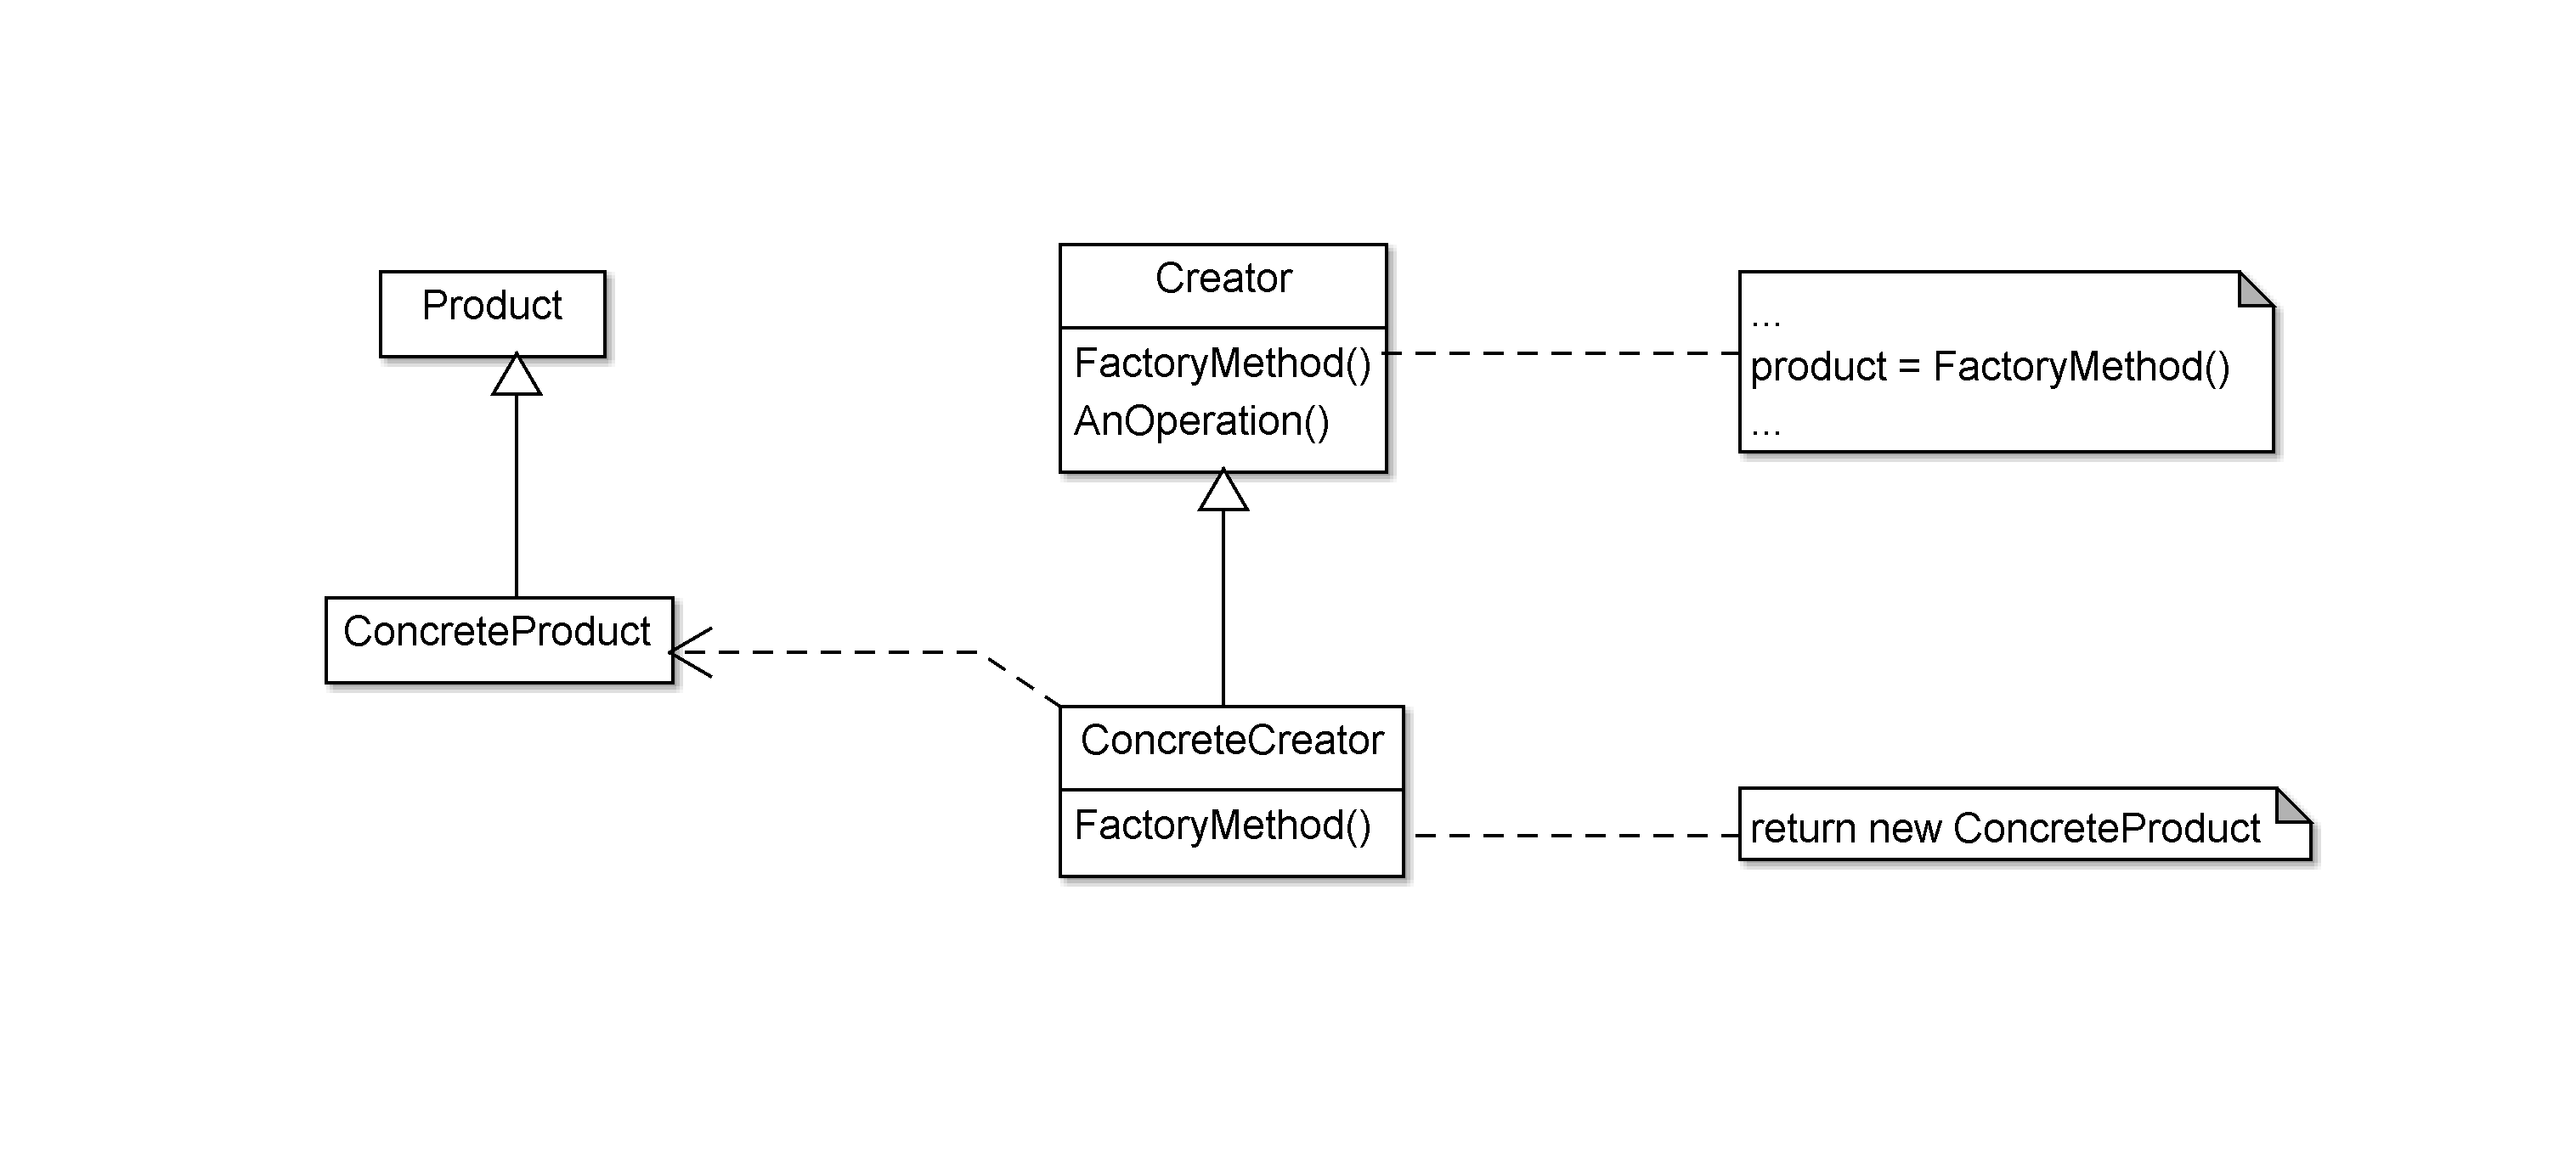
\includegraphics[width=15cm,keepaspectratio]{factory_method.png}
\end{figure}

A gyártó művelet implementálásához általában szükség van egy absztrakt gyártó osztályra, ha a példányosítandó osztálynak is van interfész osztálya. A kliens kód ezt az gyártó interfészt fogja használni. Az absztrakt gyártót megvalósító osztály  fogja a konkrét objektumot példányosítani, majd visszaadni azt a hívónak.
\subsection{Lekérdezés}
A probléma akkor adódik, ha a programban nem intuitív, hogy egy osztályt mi alapján lehet létrehozni. Jellemzően, ha egy osztály példányosítását egy delegált osztályon keresztül szeretnénk elérhetővé tenni, akkor annak valamennyi konstruktorát priváttá érdemes definiálni. Ezzel elkerülhetők olyan hibák, amelyek például más osztályok függőségéből adódnak. Azonban egy olyan kódbázisban, ahol nem egyértelmű osztályok létrehozása, mert a hozzá tartozó gyártó egy másik modulban, projektben található, akkor ennek felkutatása rengeteg időt felemészt a programozó idejéből. Egy megfelelő lekérdezéssel viszont gyorsan meg lehet találni ezeket a gyártó osztályokat.
\par  Tehát, van egy osztály definíciónk (aminek privát konstruktora van), és keressük azt az osztályt, aminek van olyan függvénye, hogy egy ilyen típusú objektummal tér vissza. 
\begin{verbatim}
factory_method(ConcreteProduct) := class {
   function {
      return: ConcreteProduct
   }
}
\end{verbatim}
\par Ezek a feltételek azonban még nem szűkítik le a találatok listáját, hogy könnyű legyen a megfelelő osztályt megtalálni. Következésképpen, ha egy osztálynak van csak egy olyan függvénye, ami a keresendő típussal tér vissza, akkor azt szintén meg lennének jelenítve a találati listában. Ha viszont a gyártó művelet tervmintából indulunk ki, akkor erősíthetünk a feltételeken. Eszerint a keresendő osztálynak van egy őse (amit a kliens kód használ), és a gyártó objektum is egy absztrakt osztályból származik (szintén a kliens kód egyszerűsítése miatt). Ezeket a további információkat felhasználva adódik az alábbi predikátum:
\begin{verbatim}
factory_method(Product, ConcreteProduct) := class {
   inherit: class {
      @abstract
      function { 
         return: Product 
      }
   }

   function {
      return: ConcreteProduct
   }
}
\end{verbatim}
\par A predikátum használatával generikussá, újra felhasználhatóvá tehető ez a típusú lekérdezés. A predikátum két paramétere az ismert osztály (\textit{ConcreteProduct}), amiből szeretnénk objektumot létrehozni és annak az ősosztály (\textit{Product}). A lekérdezésben az \textit{inherit} attribútummal erősítve a feltételeket, egy szűkített listából gyorsan megkapható a keresett osztály. Ezzel az lett megadva, hogy az interfészként szolgáló ősosztálynak is van olyan metódusa, amivel előállítható az objektum. Következésképpen, elhagytuk a találatok listájából például az olyan osztályokat, aminek van csak \textit{getter} tagfüggvény miatt van a keresendő típussal visszatérő függvénye.
\section{Átalakító osztály keresése}
Egy másik fontos területe a tervmintáknak az úgynevezett szerkezeti minták \cite{design_patterns}. Ezek a minták arra szolgálnak, hogy több objektumból összetett, nagyobb szerkezeteket hozzunk létre (általában új funkcionalitást is kapva). Egy ilyen tervminta az átalakító (vagy más néven \textit{wrapper}), amely egy osztály felületét változtatja meg a kliens által elvártra. Az örökölt (\textit{legacy}) kódban gyakran előfordulnak átalakító osztályok, ezzel elkerülve, hogy teljesen újra kelljen írni már meglévő osztályokat. Viszont ha a programozó csak a régi kódot ismeri, és nem tud az átalakító osztály definíciójáról, akkor ő is implementálni fog egy átalakítót az új felület eléréséhez. Ez több szempontból is hibákhoz vezethet: például mindkét átalakítót változtatni kell, ha a felület megváltozik, azaz mindkettőt karbantartani kell. Újrafelhasználhatóság szempontjából is érdemes a kódbázisban megkeresni az átalakító osztályokat és azokat használni.
\subsection{Átalakító tervminta}
Az átalakítóval olyan osztályok is tudnak egymással kommunikálni, kapcsolatot létesíteni, amelyek az eltérő felületük miatt nem lennének rá képesek. Több esetben is használható ez a minta. Az egyik, amikor meglévő osztályt szeretnénk használni, de felülete nem illeszkedik az igényekhez. Létezik olyan eset is, amikor több osztályt akarunk használni, de nem akarjuk származtatással átalakítani a felületüket. Ekkor egy átalakító objektummal megváltoztatható a szülő objektum felülete.
\begin{figure}
	\caption{Átalakító tervminta UML diagram}
	\centering
	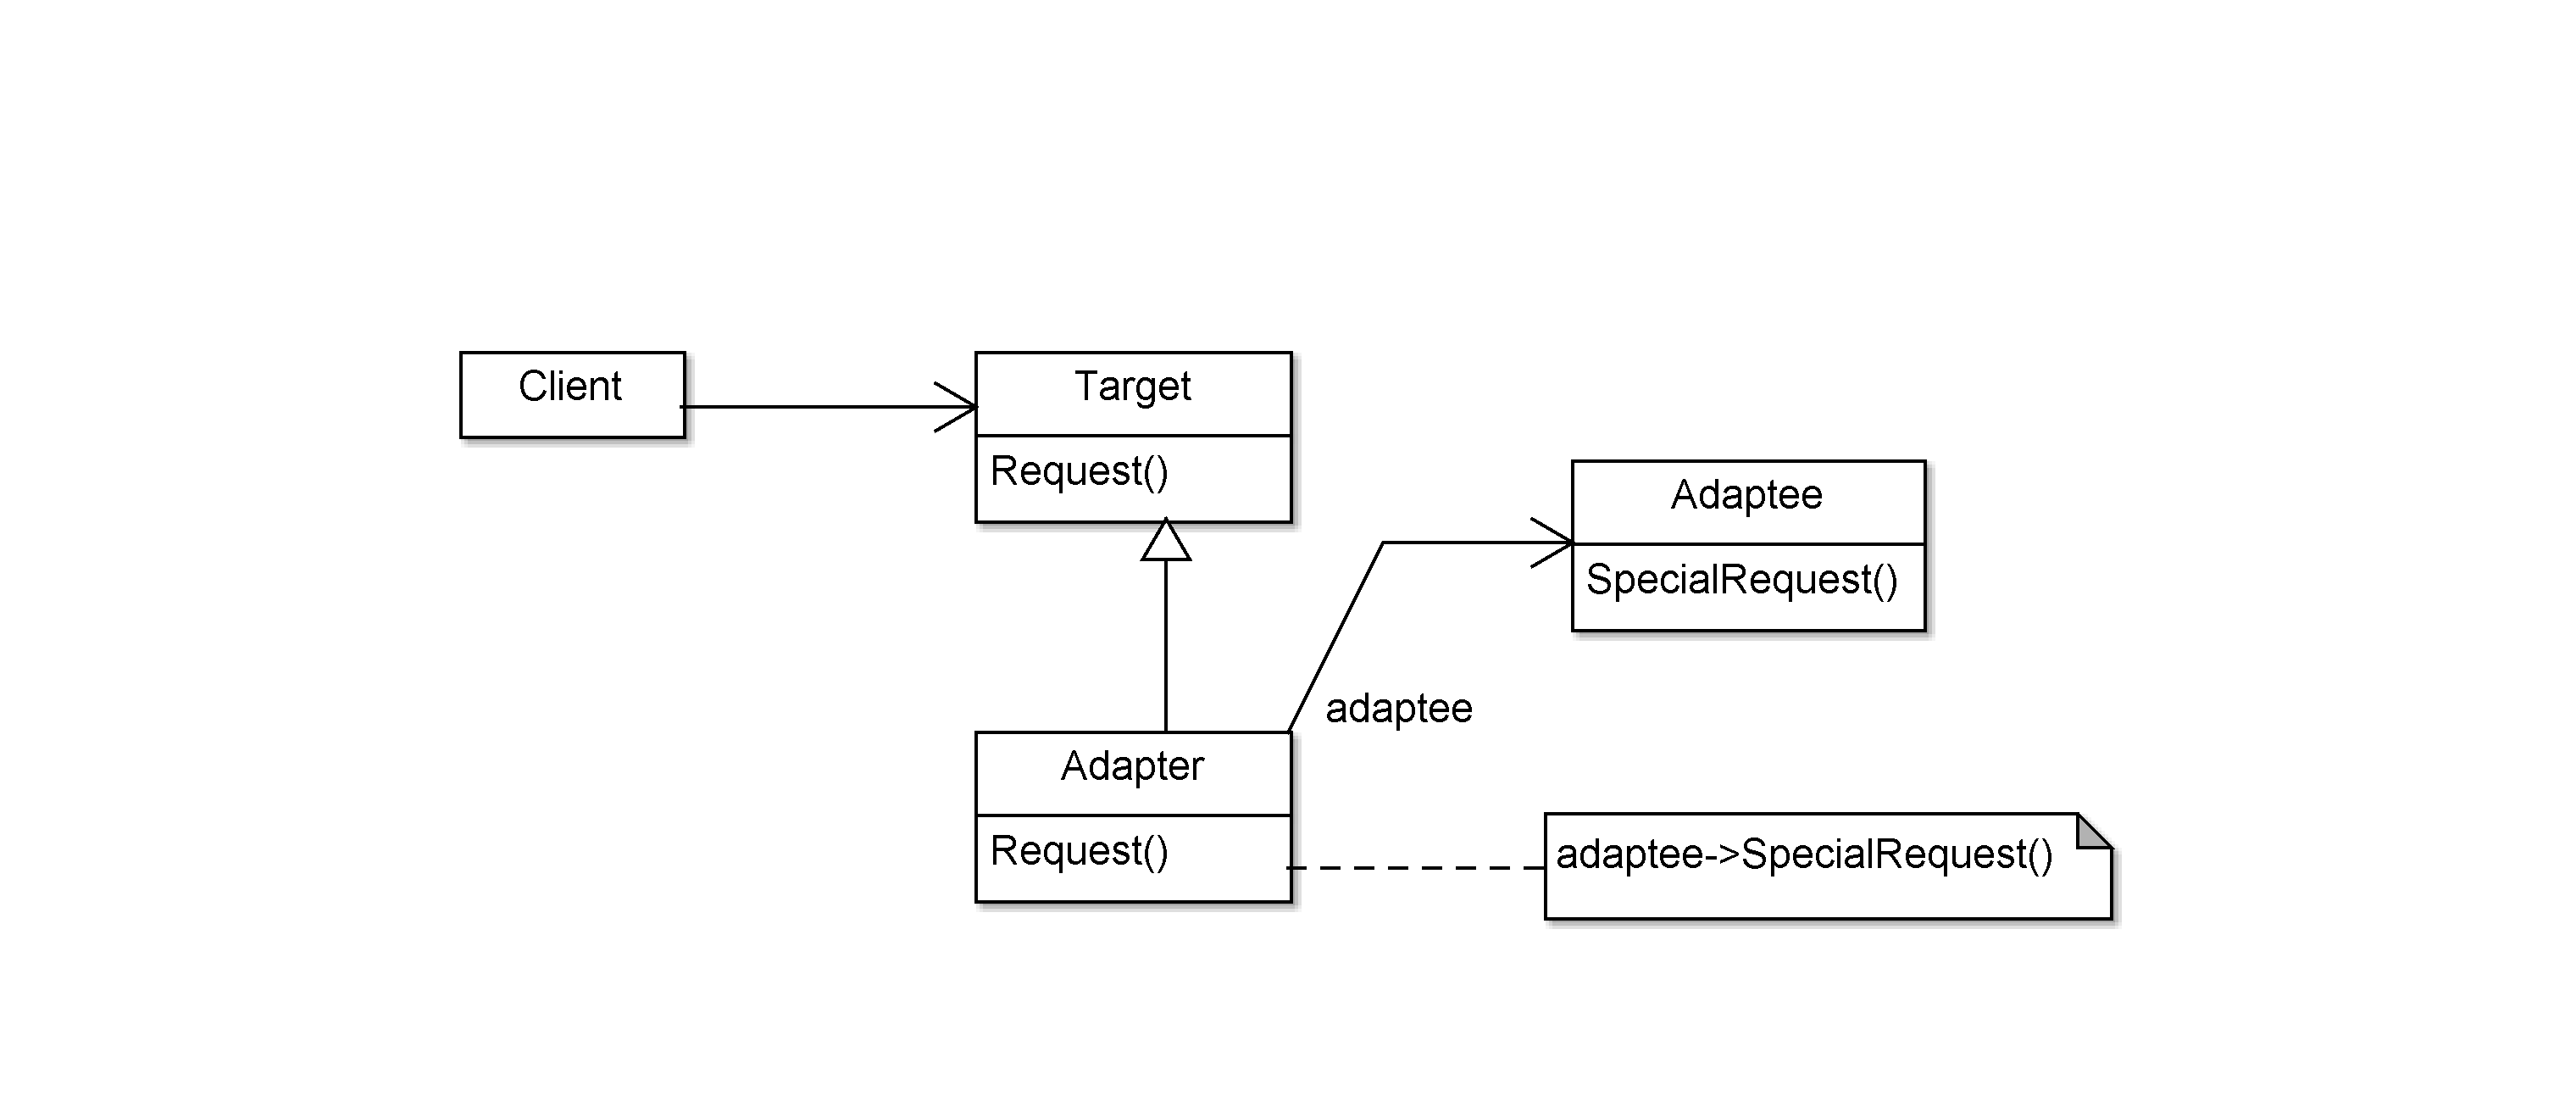
\includegraphics[width=15cm,keepaspectratio]{adapter.png}
\end{figure}
\par Az átalakító tervmintát úgy lehet implementálni, hogy az egyik komponenst becsomagoljuk egy olyan osztályba, amivel már tud kommunikálni a másik osztály. A becsomagoló osztályba aggregáljuk az egyik osztályt példányát, majd az interfész függvényeket ennek a példány tagfüggvényeinek hívásaival implementáljuk.
\subsection{Lekérdezés}
A lekérdezéshez az objektum átalakító osztályt határozzuk meg. Mivel a "régi" kódból ismerjük az osztályt, ezért annak a neve paraméterként szolgál a predikátum definíciójában. Mint az előző esettanulmánynál, úgy itt is a predikátummal (az újrafelhasználhatóságot szem előtt tartva) lehet leírni keresendő osztályokat. Az átalakítóval kapcsolatban viszont csak annyi információ áll rendelkezésre, hogy annak az adattagja az átalakított objektum, illetve rendelkezik valamennyi számú, szignatúrájú tagfüggvénnyel. Értelem szerűen az utóbbi feltételt nem lehetséges definiálni a lekérdező nyelv segítségével. Azonban az adattagra tehetünk megszorítást: mivel az átalakított osztályon kívül más objektumot nem aggregál az átalakító, így megadható további szűrő feltételnek, hogy az átalakított objektum az egyedüli adattag az osztályban.
\begin{verbatim}
wrapper(Adaptee) := class {
   variable { 
      type: Adaptee
      @only
   }
}
\end{verbatim}
\par Az \textit{only} predikátumot felhasználva kapjuk az átalakító osztály lekérdezéshez szükséges definíciót. Egy olyan osztály megtalálása a cél, aminek csak egyetlen adattagja van, az pedig az argumentumként megadott átalakítani kívánt osztály.

\chapter{Konklúzió}

\begin{thebibliography}{99}
	\bibitem{jtl} T. Cohen, J. Y. Gil, and I. Maman. JTL: The Java tools
	language. In OOPSLA, 2006.
	
	\bibitem{dotql} O. de Moor, M. Verbaere, and E. Hajiyev. Keynote address:
	.QL for source code analysis. In SCAM, 2007.
	
	\bibitem{soul} C. De Roover, C. Noguera, A. Kellens, and V. Jonckers. The
	SOUL tool suite for querying programs in symbiosis with
	Eclipse. In PPPJ, 2011.
	
	\bibitem{jquery} D. Janzen and K. De Volder. Navigating and querying code
	without getting lost. In AOSD, 2003.
	
	\bibitem{pql}  M. Martin, V. B. Livshits, and M. S. Lam, “Finding application
	errors and security flaws using PQL: a program query language,” 
	in Object Oriented Programming, Systems, Languages and Applications (OOPSLA’07). ACM, 2005, pp.	365–383.
	
	\bibitem{json}Bray, Tim. "The javascript object notation (json) data interchange format." (2014).
	
	\bibitem{design_patterns} Vlissides, John, et al. "Design patterns: Elements of reusable object-oriented software." Reading: Addison-Wesley 49.120 (1995): 11.
	
	\bibitem{eqn_1}E. W. Dijkstra and C. S. Scholten. Predicate Calculus and
	Program Semantics. Texts and Monographs in Computer
	Science. Springer Verlag, 1990
	
	\bibitem{eqn_2}A. Kaldewaij. The Derivation of Algorithms. Prentice Hall,
	1990
	
	\bibitem{rule_of_three} $http://en.cppreference.com/w/cpp/language/rule_of_three$ , 2017.05.09
	
	\bibitem{xpath} Berglund, Anders, et al. "Xml path language (xpath)." World Wide Web Consortium (W3C) (2003).
	
\end{thebibliography}
	
\end{document}